\documentclass[shownotes, xcolor = table]{beamer}

\usepackage{xeCJK}
\usepackage{fontspec}
\usepackage{comment}

\usetheme{CambridgeUS} % try Madrid
\usecolortheme{beaver} % try beaver, dolphin, seahorse
\usefonttheme[onlymath]{serif} % try "professionalfonts"
\setCJKmainfont{Microsoft YaHei} % try SimSun

\usepackage{amsmath, amsfonts, amssymb, mathtools, pifont}
\newcommand{\cmark}{\ding{51}}%
\newcommand{\xmark}{\ding{55}}%
\def\checkmark{\tikz\fill[scale=0.5](0,.35) -- (.25,0) -- (1,.7) -- (.25,.15) -- cycle;} 

\usepackage{graphicx, subcaption}
% textpos for textblock (putting objects at specified positions)
% \usepackage[absolute, overlay]{textpos}  
\usepackage{adjustbox}

\usepackage[framemethod=TikZ]{mdframed}

\usepackage[normalem]{ulem} % strike through text
\newcommand{\soutthick}[1]{%
    \renewcommand{\ULthickness}{2.0pt}%
       \sout{#1}%
    \renewcommand{\ULthickness}{.4pt}% Resetting to ulem default
}

% \usepackage{biblatex}
% \addbibresource{phd-defense-report.bib}

\setbeamersize{text margin left = 2em, text margin right = 1em}
\setbeamercolor{footnote mark}{fg = teal}
\setbeamertemplate{itemize items}[default]
\setbeamertemplate{enumerate items}[default]

\usepackage{tikz}
\usetikzlibrary{arrows.meta, shapes, positioning, calc, backgrounds, fit}

\theoremstyle{plain}
\newtheorem{cdef}{定义}[section]
\newtheorem{ctheorem}{定理}[section]
\newtheorem{cquestion}{问题:}[section]

% for tables
\usepackage{multirow}
\newcommand{\innercell}[2]{\begin{tabular}{@{}#1@{}}#2\end{tabular}}

% for fig without caption: #1: width/size; #2: fig file
\newcommand{\fignocaption}[2]{
  \begin{figure}[htp]
    \centering
    \includegraphics[#1]{#2}
  \end{figure}
}

% for fig without caption: #1: width/size; #2: fig file; #3: fig caption
\newcommand{\fig}[3]{
  \begin{figure}[htp]
    \centering
      \includegraphics[#1]{#2}
      \caption{#3}
  \end{figure}
}

% for cite: #1: author; #2: conference #3: year
\newcommand{\citeinbeamer}[3]{{\tiny{\textcolor{blue}{[#1@#2'#3]}}}}

\newcommand{\term}[1]{\textcolor{blue}{\scriptsize (#1)}}
\newcommand{\set}[1]{\{#1\}}
\newcommand{\question}[1]{\textcolor{red}{\large #1}}
\newcommand{\answer}[1]{\textcolor{blue}{\bf #1}}
\newcommand{\alertred}[1]{\textcolor{red}{#1}}
\newcommand{\alertblue}[1]{\textcolor{blue}{#1}}
\newcommand{\todo}[1]{\textcolor{red}{\textbf{TODO:} #1}}
\newcommand{\mathbfblue}[1]{\textcolor{blue}{$\mathbf{#1}$}}

\newcommand{\papertitle}{分布数据一致性技术研究}
\newcommand{\idea}{``多样化, 可调节; 精细化, 可度量''}
\newcommand{\ideadt}{``多样化, 可调节''}
\newcommand{\idearm}{``精细化, 可度量''}
%%%%%%%%%%%%%%%%%%%%%%%%%%%%%%%%%%%%%%%%%%%%%%%%%%%%%%%%%%%%%%%%%%%%%%%%%%%%%%%%	
\title[\papertitle]{\papertitle}
\subtitle{}

\author[魏恒峰]{魏恒峰 \\导师: 吕建 \hspace{0.20cm} 黄宇}
\institute{南京大学软件所}
\date{\today}

\AtBeginSection[]{
  \begin{frame}[noframenumbering, plain]
    \frametitle{\papertitle}
    \tableofcontents[currentsection, sectionstyle=show/shaded, subsectionstyle=show/show/hide]
  \end{frame}
}

% Delete this, if you do not want the table of contents to pop up 
% at the beginning of each subsection:
\AtBeginSubsection[]{
  \begin{frame}[noframenumbering, plain]
    \frametitle{\papertitle}
      \tableofcontents[currentsection, sectionstyle=show/shaded, subsectionstyle=show/shaded/hide]
  \end{frame}
}

% \bibliography{phd-defense-report.bib}
%%%%%%%%%%%%%%%%%%%%
\begin{document}

\renewcommand\figurename{图} 
\renewcommand\tablename{表} 

% mdf: mdframed; #1: frame color; #2: frame title color; #3: frame title; #4: text color; #5: text
\newcommand{\mdf}[5]{
\begin{mdframed}[frametitle={
  \tikz[baseline = (current bounding box.east), outer sep = 0pt]
  \node[anchor = east, rectangle, fill = #1!20, font = \small]{\strut \textcolor{#2}{#3:}};},
  innertopmargin = 2pt, linecolor = #1!20, linewidth = 2pt, topline = true,
  frametitleaboveskip=\dimexpr-\ht\strutbox\relax]
  \begin{center}
	\textcolor{#4}{#5}
  \end{center}
\end{mdframed}
}

\maketitle

\begin{frame}[noframenumbering, plain]
  \frametitle{\papertitle}
  \tableofcontents[currentsection, sectionstyle=show, subsectionstyle=show/show/hide]
\end{frame}

% \begin{frame}[noframenumbering, plain]
%   \frametitle{分布数据一致性理论与技术研究}
%   \begin{enumerate}
%     \setlength{\itemsep}{15pt}
% 	\item {\bf 研究背景:} {\footnotesize 分布数据}
% 	\item \textcolor{blue}{研究问题:} {\footnotesize 数据一致性}
% 	\item \textcolor{blue}{研究方法:} {\footnotesize 理论模型 + 技术框架}
% 	\item \textcolor{blue}{主要工作:} {\footnotesize VPC + PA2AM + RVSI}
% 	\item \textcolor{blue}{未来工作}
%   \end{enumerate}
% \end{frame}

\section{研究背景}

%%%%%%%%%%%%%%%
\begin{frame}{分布式应用}
  \fignocaption{width = 0.50\textwidth}{figures/sina-weibo.pdf}

  \begin{columns}
	\column{0.50\textwidth}
	新浪微博社交网站 \footnotemark:
	\begin{itemize}
	  \item 日均用户近一亿
	  \item 日均消息近一亿条
	\end{itemize}

	\column{0.50\textwidth}
	底层数据服务系统特性需求:
	\begin{itemize}
	  \item 低延迟, 高可用性 (4个9 \footnotemark)
	  \item 高容错性, 高可扩展性
	\end{itemize}
  \end{columns}
  
  \footnotetext[1]{2015第三季度; 数据来自 China Internet Watch.}
  \footnotetext[2]{数据来自 InfoQ.}
\end{frame}
%%%%%%%%%%%%%%%
\begin{frame}{分布数据}
  \fignocaption{width = 0.60\textwidth}{figures/distributed-data.pdf}

  \only<1-3>{应用数据:} \uncover<4->{ \textcolor{red}{分布数据:}}
  \begin{enumerate}
	\item<2-> 分区 \term{partition}: 水平扩展
	\item<3-> 副本 \term{replication}: 就近访问, 容灾备份
  \end{enumerate}
\end{frame}
%%%%%%%%%%%%%%%
\begin{frame}{分布共享数据服务}
  \fignocaption{width = 0.50\textwidth}{figures/sina-weibo.pdf}

  \begin{center}
	分布共享数据服务 \term{中间件}:
	\vspace{0.50cm}

	屏蔽底层数据分布性\; 提供共享数据抽象\; 简化上层应用开发
  \end{center}
\end{frame}
%%%%%%%%%%%%%%%
\begin{frame}{分布共享数据服务典型应用 (I)}
  \fig{width = 0.55\textwidth}{figures/dsss.pdf}
  {分布式存储系统 (\textcolor{blue}{\scriptsize 开源 [左]} \& \textcolor{red}{\scriptsize 商用 [右]}).}

  % \begin{description}
  %   \item[低延迟:] 就近访问副本数据
  %   \item[高可用性, 高容错性:] 备份容灾 
  % \end{description}
\end{frame}
%%%%%%%%%%%%%%%
\begin{frame}{分布共享数据服务典型应用 (II)}
  \fig{width = 0.75\textwidth}{figures/file-share.pdf}
  {个人多设备文件共享 {(\textcolor{blue}{\scriptsize [基于云] C/S 结构 [左]} \& 
  \textcolor{red}{\scriptsize P2P 结构 [右]}).}}

  \begin{description}
    \item[功能需求:] 文件副本 \citeinbeamer{Strauss}{MIT Thesis}{10}
    \item[网络断连:] 备份容灾; 离线可用
  \end{description}
\end{frame}
%%%%%%%%%%%%%%%
% \begin{frame}{分布副本数据的典型应用 (三)}
%   \fig{width = 0.80\textwidth}{figures/coordination.pdf}
%   {分布式协同应用(上)及服务(下).}
% 
%   分布式协同服务需求 \citeinbeamer{Burrows}{OSDI}{06} vs. ``副本技术'':
%   \begin{description}
%     \item[高性能:] 低延迟就近``读''副本 \citeinbeamer{Yahoo!}{USENIXATC}{10}
%     \item[高可靠性:] 避免单点协同故障
%   \end{description}
% \end{frame}
%%%%%%%%%%%%%%%

\section{研究问题}

%%%%%%%%%%%%%%%
% \begin{frame}{分布数据一致性问题}
%   \graphicspath{{tikz-in-beamer/}}
%   \begin{figure}[h!]
%     \centering
%     \begin{adjustbox}{max totalsize = {0.50\textwidth}{1.00\textheight}, center}
% 	  % File: beamer overlay for distributed-data.tex
% Created: Nov. 2, 2016

\begin{tikzpicture}[rc/.style = {circle, minimum size = 4cm, fill = red},
  br/.style = {rectangle, rounded corners, minimum size = 4cm, fill = blue},
  gs/.style = {shape = star, scale = 8, star points = 5, star point ratio = 1.65, fill = green},
  dash pattern = {on 20pt off 10pt},
  partition/.style = {draw, lightgray, line width = 8pt},
  replication/.style = {draw, dash phase = 0pt, line width = 10pt, #1},
  access/.style = {draw, > = stealth, <->, dash phase = 0pt, line width = 6pt, brown}]

  \begin{pgfonlayer}{background}
	\node[opacity = 0.80] (map) {\includegraphics[scale = 0.50]{figs/world-map-logo.jpg}};
  \end{pgfonlayer}

  % shared data
  \begin{scope}[yshift = -18cm]
	\node[rc] (circ) {};
	\node[br, left = 2cm of circ] (rect) {};
	\node[gs, right = 2cm of circ] (st) {};

	\begin{pgfonlayer}{background}
	  \node[rectangle, rounded corners, fill = black!30, fit = (circ) (rect) (st), inner sep = 5pt, 
		label = {[font = \fontsize{65}{70}\sffamily\bfseries] below : Application Data}] (data) {};
	  \end{pgfonlayer}
	\end{scope}

	% partition
	\node[rc] (circ1) at (20, 10) {};
	\node[br] (rect1) at (-25, 10) {};
	\node[gs] (st1) at (28, -12) {};

	\draw[partition] (circ) to (circ1);
	\draw[partition] (rect) to (rect1);
	\draw[partition] (st) to (st1);


	% replication
	\node[rc] (circ2) at (-15, -10) {};
	\node[rc] (circ3) at (-10, 18) {};

	\node[br] (rect2) at (10, 12) {};

	\node[gs] (st2) at (0,0) {};
	\node[gs] (st3) at (20, 5) {};

	\path[replication = {red}] (circ1) to (circ2) 
	(circ2) to (circ3)
	(circ3) to (circ1);

	\path[replication = {blue}] (rect1) to (rect2);

	\path[replication = {green}] (st1) to (st2) 
	(st2) to (st3)
	(st3) to (st1);


  \uncover<2->{
  % sina-weibo clients
  \def\SCALE{0.15}
  \node[] (sina1) at (-25, 0) {
\includegraphics[scale = \SCALE]{figs/sina-weibo.png}};
  \node[] (sina2) at (10, 5) {
\includegraphics[scale = \SCALE]{figs/sina-weibo.png}};
  \node[] (sina3) at (5, -10) {
\includegraphics[scale = \SCALE]{figs/sina-weibo.png}};

  % access
  \path[every edge/.append style = {access}] (sina1) edge (rect1)
  				(sina1) edge (circ2)
				(sina2) edge (rect2)
				(sina2) edge (st2)
				(sina3) edge (circ1)
				(sina3) edge (st2);
  }
\end{tikzpicture}

%     \end{adjustbox}
%   \end{figure}
% 
%   \uncover<2->{
% 	\textcolor{red}{分布数据 \term{distributed data}} $\Leftarrow$ 共享 (集中式) 数据 \term{shared data}:}
%   \vspace{0.30cm}
%   \begin{description}
% 	\item<3->[上层应用:] 分布数据的语义是什么? 如何``方便''地使用分布数据?
% 	\item<4->[数据副本:] 以何种顺序应用更新? 对应用提供什么保证?
%   \end{description}
% \end{frame}
% %%%%%%%%%%%%%%%
% \begin{frame}{分布数据一致性问题}
%   \begin{figure}[h!]
%     \centering
%     \begin{adjustbox}{max totalsize = {0.70\textwidth}{1.00\textheight}, center}
% 	  % This example is from WYATT LLOYD@CACM14 (Don't Settle For Eventual Consistency)
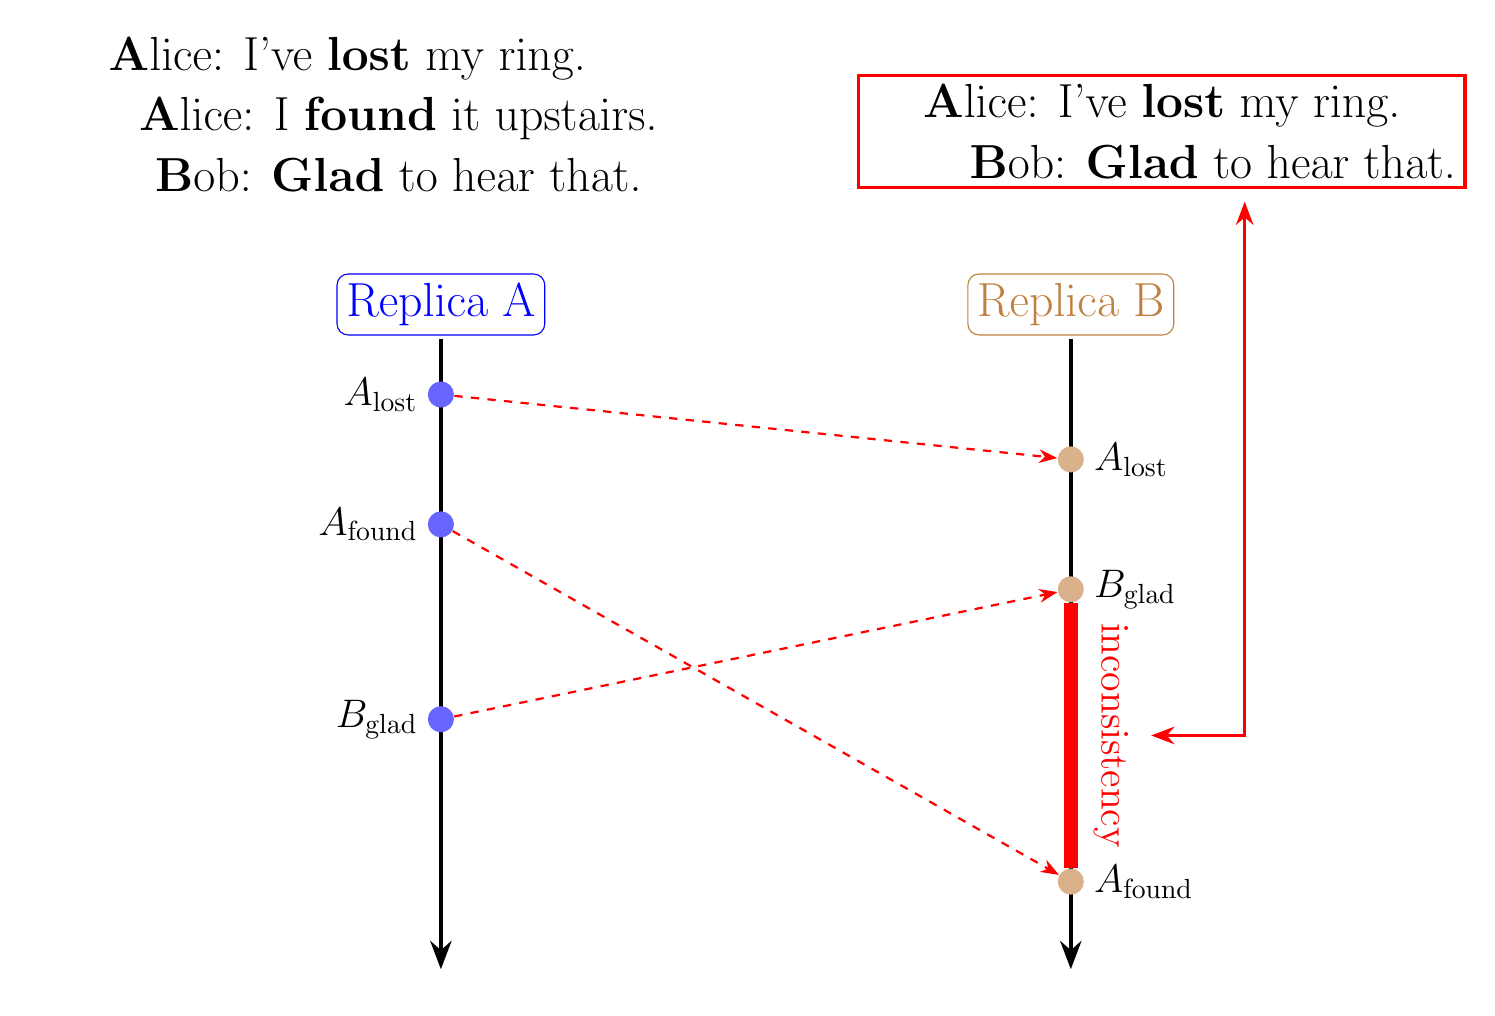
\begin{tikzpicture}
  % replica A at west coast
  \begin{scope}[font = \Large, wnode/.style = {fill = blue!60, circle}]
    \node (west-start) [] at (0,0) {};
    \node (west-end) [below = 8cm of west-start] {};

	\uncover<2->{
    \draw [>=Stealth, ->, ultra thick] (west-start) to (west-end);

    \node (west-a-lost) [wnode, label = 180: $A_{\textrm{lost}}$] at ($(west-start) !0.10! (west-end)$) {};
    \node (west-a-found) [wnode, label = 180: $A_{\textrm{found}}$] at ($(west-start) !0.30! 
    (west-end)$) {};
    \node (west-b-glad) [wnode, label = 180: $B_{\textrm{glad}}$] at ($(west-start) !0.60! (west-end)$) {};

    % text
    \node (west-text) [above left = 1.5cm and -3.00cm of west-start, align = center, font = \LARGE] {{\bf A}lice: I've {\bf lost} my ring.
    \\ $\qquad$ {\bf A}lice: I {\bf found} it upstairs. 
    \\ $\qquad$ {\bf B}ob: {\bf Glad} to hear that.};
  }

    % replica A at west coast
	\uncover<1->{
	  \node (replicaA) [above = -0.20cm of west-start, font = \LARGE, draw = blue, rectangle, rounded corners] {\textcolor{blue}{Replica A}};}
  \end{scope}

  % replica B at east coast
  \begin{scope}[xshift = 8.0cm, font = \Large, enode/.style = {fill = brown!60, circle}]
    \node (east-start) [] at (0,0) {};
    \node (east-end) [below = 8cm of east-start] {};
	\uncover<3->{
	\draw [>=Stealth, ->, ultra thick] (east-start) to (east-end);

    \node (east-a-lost) [enode, label = 0: $A_{\textrm{lost}}$] at ($(east-start) !0.20! (east-end)$) {};
    \node (east-b-glad) [enode, label = 0: $B_{\textrm{glad}}$] at ($(east-start) !0.40! 
    (east-end)$) {};
    \node (east-a-found) [enode, label = 0: $A_{\textrm{found}}$] at ($(east-start) !0.85! (east-end)$) {};

  % message-passing and message-reordering
  \begin{scope}[>=Stealth, ->, thick, dashed, red]
    \draw (west-a-lost) to (east-a-lost);
    \draw (west-a-found) to (east-a-found);
    \draw (west-b-glad) to (east-b-glad);
  \end{scope}
  }
    
    % replica B at east coast
	\uncover<1->{
	  \node (replicaB) [above = -0.20cm of east-start, font = \LARGE, draw = brown, rectangle, rounded corners] {\textcolor{brown}{Replica B}};}
  \end{scope}

  \uncover<4->{
  \begin{scope}[font = \Large]
    % data inconsistency in replicaB
    \draw [line width = 5pt, red] (east-b-glad) -- (east-a-found) 
	node (inconsistency) [above, midway, sloped, outer sep = 5pt] {inconsistency};
    % text
    \node (east-text) [draw = red, very thick, rectangle, 
	above right = 1.5cm and -3.00cm of east-start, align = center, font = \LARGE, 
	  outer sep = 5pt] 
	  {{\bf A}lice: I've {\bf lost} my ring.  
	  \\ $\qquad$ {\bf B}ob: {\bf Glad} to hear that.};
	% link
    \draw [>=Stealth, very thick, red, <->] 
	  (inconsistency) -| ($(east-text.south) + (30pt,0)$);
  \end{scope}
  }
\end{tikzpicture}

%     \end{adjustbox}
% 	\caption{社交网络中, 消息-评论乱序 \citeinbeamer{Lloyd}{CACM}{14}.}
%   \end{figure}
% \end{frame}
%%%%%%%%%%%%%%%
\begin{frame}{分布数据一致性问题}
  \graphicspath{{tikz-in-beamer/}}
  \begin{figure}[h!]
    \centering
    \begin{adjustbox}{max totalsize = {0.90\textwidth}{1.00\textheight}, center}
	  \begin{tikzpicture}[font = \Large]
  \node (share) [label = {below:共享数据}] {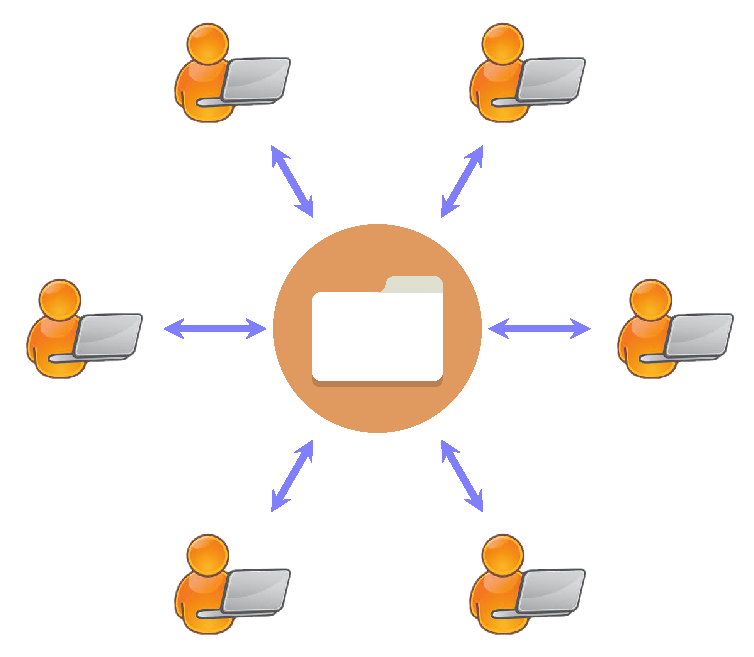
\includegraphics[height = 4cm]{shared-data-clients.pdf}};
  \node (dist) [label = {below:分布数据}, right = 9.0cm of share] {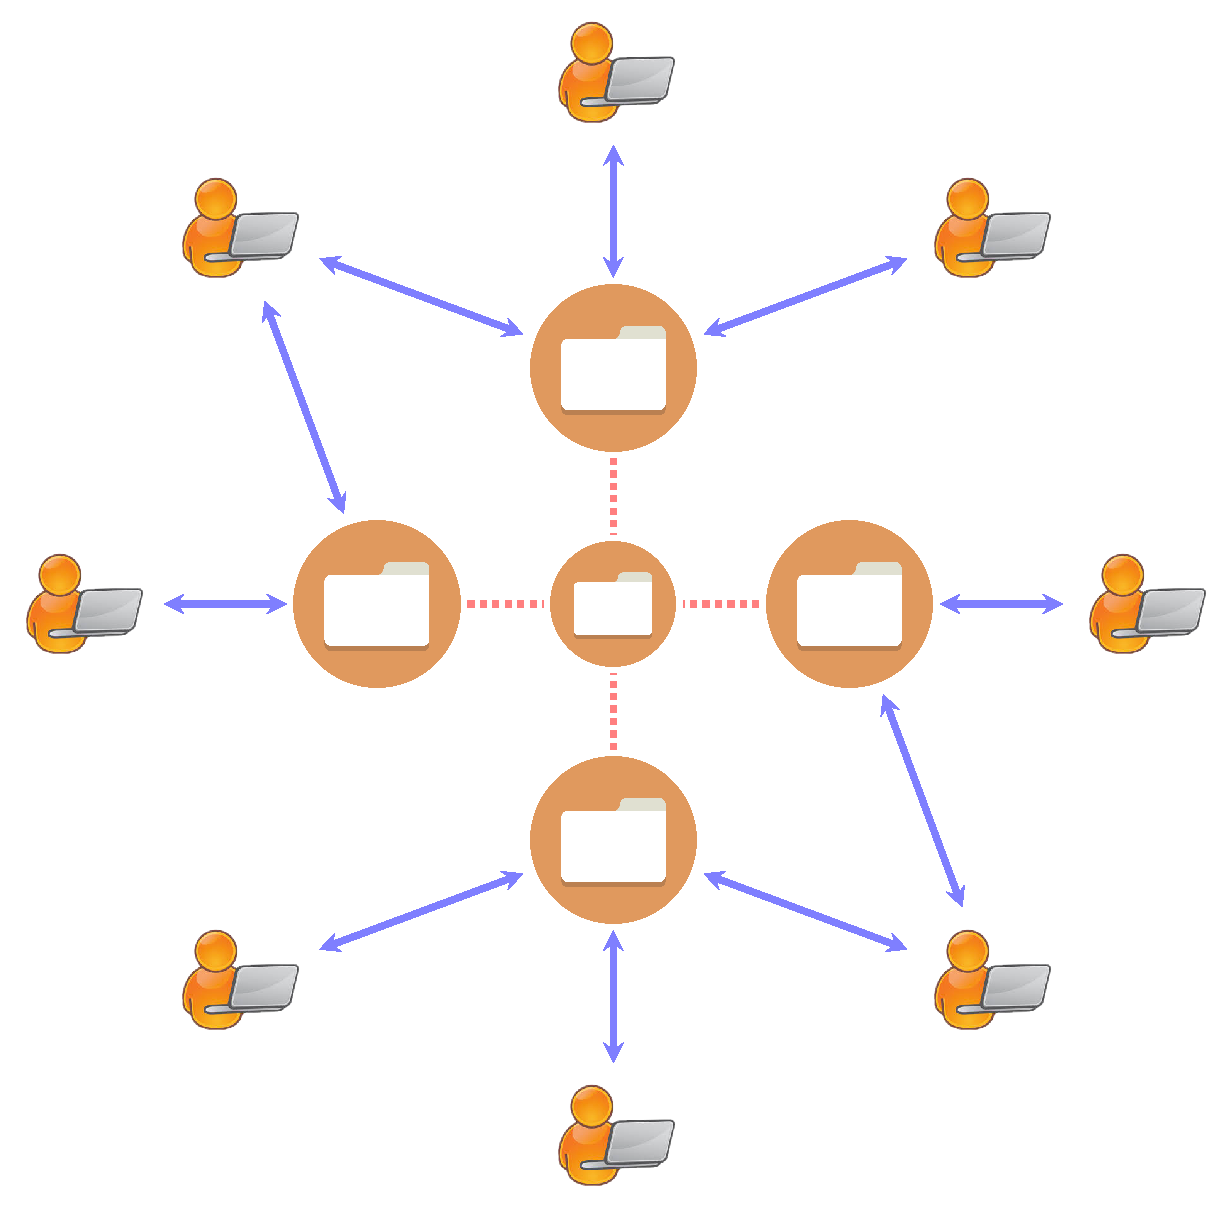
\includegraphics[height = 4.5cm]{distributed-data-clients.pdf}};

  % from (share) to (dist)
  \uncover<2->{
  \draw [-Implies, brown, line width = 1pt, double distance = 2pt, bend right = 35] (share) to node [black, sloped, below = 8pt] {分布数据一致性问题} (dist);
  }

  % from (dist) to (share)
  \uncover<4->{
  \draw [-Implies, brown, line width = 1pt, double distance = 2pt, bend right = 35] (dist) to node () [black, sloped, above = 8pt] 
  {像访问共享数据一样访问分布数据} (share);
  }

  % middleware
  \uncover<3->{
  \node (dsds) [] at ($(share.center)!0.5!(dist.center)$) {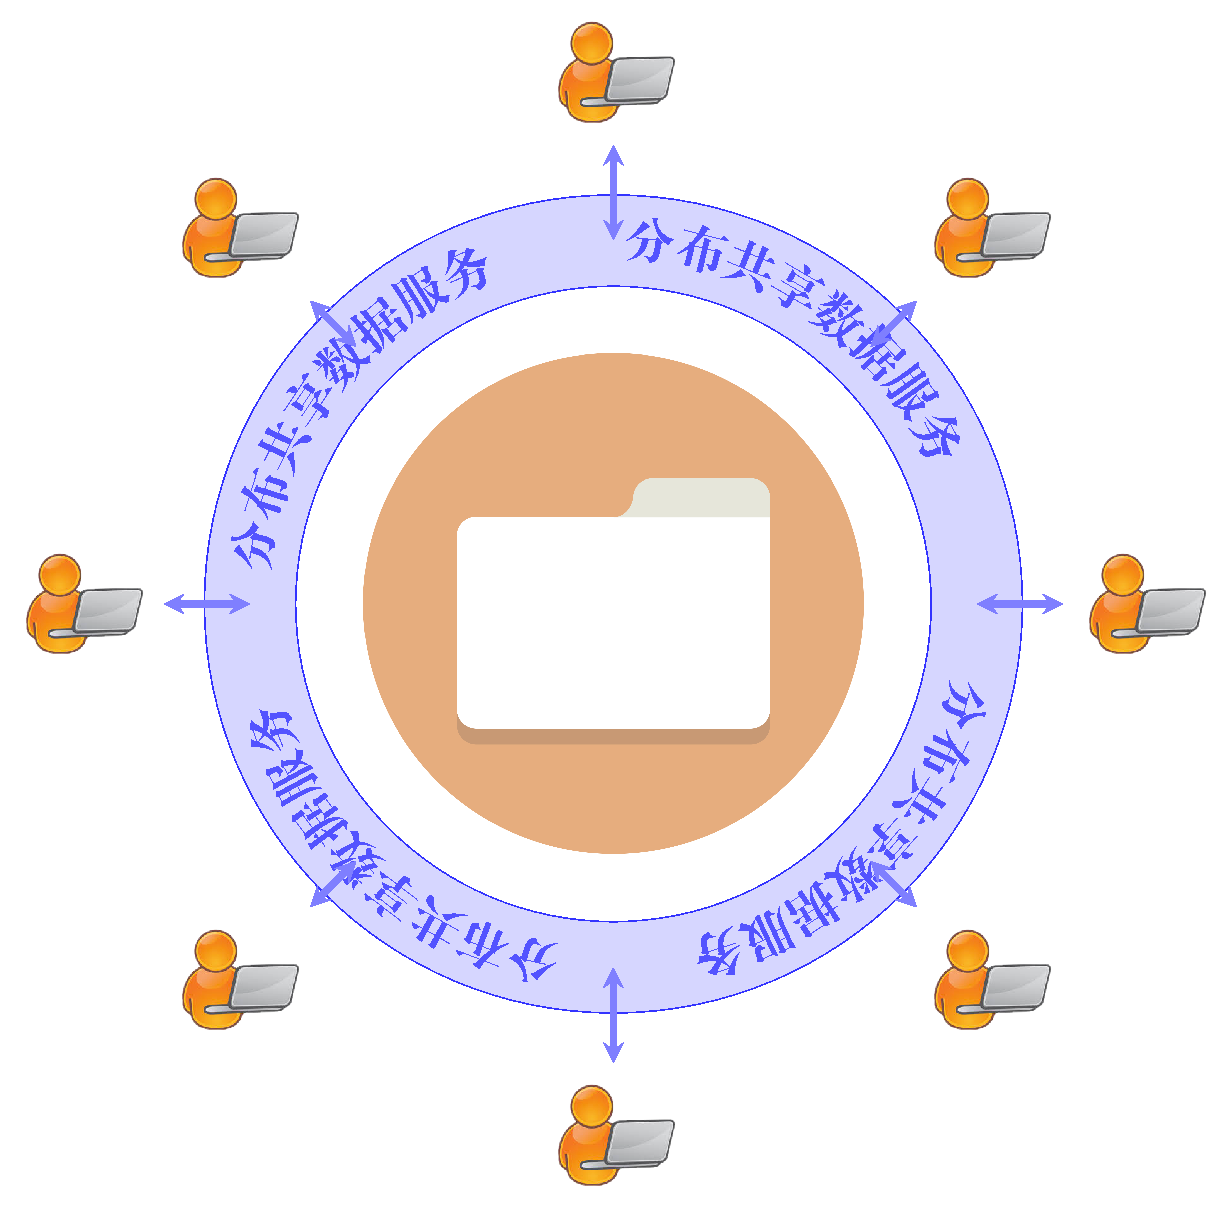
\includegraphics[height = 6cm]{distributed-shared-data-clients-chinese.pdf}};
  \draw [-Implies, blue!60, line width = 1pt, double distance = 1pt] (dist) to (dsds);
  \draw [-Implies, blue!60, line width = 1pt, double distance = 1pt] (dsds) to (share);
  }
\end{tikzpicture}
    \end{adjustbox}
  \end{figure}

  \begin{columns}
	\column{0.50\textwidth}
	  \uncover<2->{
		分布数据一致性问题 \textcolor{blue}{\small (应用视角)}:
	  \begin{itemize}
		\item 分布数据的语义是什么?
		\item 如何``方便''地使用分布数据?
	  \end{itemize}
	  }
	\column{0.50\textwidth}
	  \uncover<3->{
		分布共享数据服务 \textcolor{blue}{\small (中间件)}:
		\begin{itemize}
		  \item 屏蔽分布数据细节
		  \item 提供共享数据抽象
		\end{itemize}
	  }
  \end{columns}
\end{frame}
%%%%%%%%%%%%%%%
\begin{frame}{分布数据一致性问题}
  \begin{columns}[t]
	\column{0.40\textwidth}
	  理想情况:
	  \begin{itemize}
		\item one-size-fits-all\\一致性方案
		\item 始终观察到最新副本
	  \end{itemize}
	  \only<1-2>{
	  \begin{center}
		\textcolor{blue}{没有分布数据一致性问题}
	  \end{center}
	  }
	  \only<3->{
	  \begin{center}
		\textcolor{blue}{\soutthick{没有分布数据一致性问题}}
	  \end{center}
	  }
    \pause
	\column{0.48\textwidth}
	实际情况 (tradeoffs):
	  \fignocaption{width = 0.60\textwidth}{figures/consistency-centric-tradeoff.pdf}
  \end{columns}
  \pause
  \vspace{0.50cm}
  \begin{center}
	% \textcolor{red}{分布数据一致性问题是分布共享数据服务中的核心问题}
	\textcolor{blue}{在分布式系统中, \\以数据一致性为核心的权衡 \citeinbeamer{Guerraoui}{TCDE}{16} 使得 \\
  		分布数据一致性问题成为分布共享数据服务中的核心难题.}
  \end{center}
\end{frame}
%%%%%%%%%%%%%%%
% \begin{frame}{分布数据一致性问题举例 (I)}
%   \fig{width = 0.60\textwidth}{figures/data-inconsistency-comment-reordering.pdf}
%   {社交网络中, 消息-评论乱序 \citeinbeamer{Lloyd}{CACM}{14}.}
% \end{frame}
% %%%%%%%%%%%%%%%
% \begin{frame}{分布数据一致性问题举例 (II)}
%   \begin{figure}[h!]
%     \centering
%     \begin{adjustbox}{max totalsize = {0.65\textwidth}{0.65\textheight}, center}
%       %        File: data-inconsistency-rmw.tex
%     Created: Thu Oct 08 10:00 AM 2015 C
% Last Change: Thu Oct 08 10:00 AM 2015 C
%
\begin{tikzpicture}
  \uncover<1->{
  \begin{scope}
    % phone
    \node (phone) [] at (0,0) {
\includegraphics[scale = 0.4]{figures/phone-icon.png}};
    % tablet
    \node (tablet) [below left = 4.0cm and 3.0cm of phone] {
\includegraphics[scale = 
    0.55]{figures/tablet-icon.jpg}};
    % pc
    \node (pc) [below right = 4.0cm and 3.0cm of phone] {
\includegraphics[scale = 
    0.60]{figures/pc-icon}};
  \end{scope}
  }

    % write from pc 
  \uncover<2->{
    \begin{scope}[<->, blue, line width = 6pt, font = \huge]
      % person at pc
      \only<2>{
      \node (person-pc) [above left = -1.0cm and -2.0cm of pc] {
\includegraphics[scale = 
      0.30]{figures/person-icon}};
      }
      \draw [] (pc.west) to node [midway, sloped, above] {\textbf{1.} update file $f$} 
      (tablet.east);
      \draw [red, loosely dashed] (pc.north) to [out = 90, in = -20] node [midway, sloped, font = 
      \Huge, scale = 2]{$\times$} (phone.east);
      \draw (pc) to [loop, out = 60, in = -10, looseness = 3] node [midway, above, sloped] 
      {\textbf{1.} update file $f$} (pc);
    \end{scope}
   }


    % read from phone
   \uncover<3->{
    \begin{scope}[<->, brown, line width = 6pt, font = \huge]

      % person at phone
      \node (person-phone) [above left = -1.0cm and -2.0cm of phone] {
\includegraphics[scale = 
      0.30]{figures/person-icon}};

      \draw (phone) to [loop, out = 180, in = -100, looseness = 3] node [midway, below, sloped] 
      {\textbf{2.} read file $f$} (phone);   
    \end{scope}

    % update lost
    \node (inconsistency) [font = \huge, right = of person-phone, red] {\bf Update Lost!};
  }
\end{tikzpicture}

%     \end{adjustbox}
%     \caption{多设备文件共享时, 更新丢失 ($\#N = 3, \#W = 2, \#R = 1$).}
%   \end{figure}
% \end{frame}
%%%%%%%%%%%%%%%
\begin{frame}{分布数据一致性问题}
  \mdf{red}{red}{论文研究动机}{blue}{考虑到上述权衡, \\面向分布式系统的\\分布数据一致性理论应体现什么特性?}

  \pause
  \vspace{0.80cm}

  \begin{center}
	分布式系统设计与其应用有哪些特点,\\对分布数据一致性理论有何影响?
  \end{center}

  % 考察分布数据一致性问题研究的历史:
  % \vspace{8pt}
  % \begin{itemize}
  %   \setlength{\itemsep}{6pt}
  %   \item 核心权衡与解决方案 
  %     \pause
  %   \item 理论与系统
  % \end{itemize}
\end{frame}
%%%%%%%%%%%%%%%
\begin{frame}{多处理器系统领域中的数据一致性理论}
  \textcolor{gray}{\small (分布)} 数据一致性问题是多处理器系统领域中的传统问题:
  \vspace{0.50cm}

  \begin{figure}
	\begin{subfigure}{0.50\textwidth}
	  \centering
	  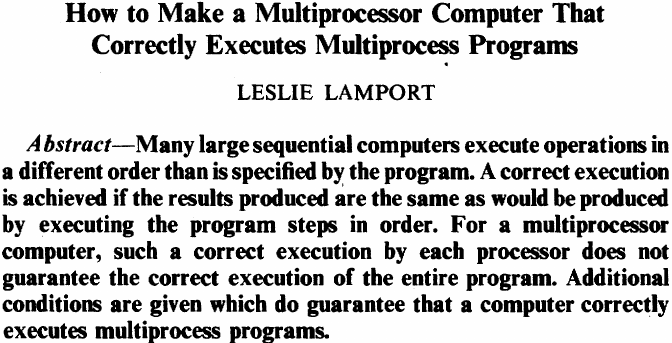
\includegraphics[width = 0.85\textwidth]{figures/lamport-paper79.png}
	  \caption{Sequential Consistency \citeinbeamer{Lamport}{TC}{79}.}
	\end{subfigure}%
	\begin{subfigure}{0.45\textwidth}
	  \centering
	  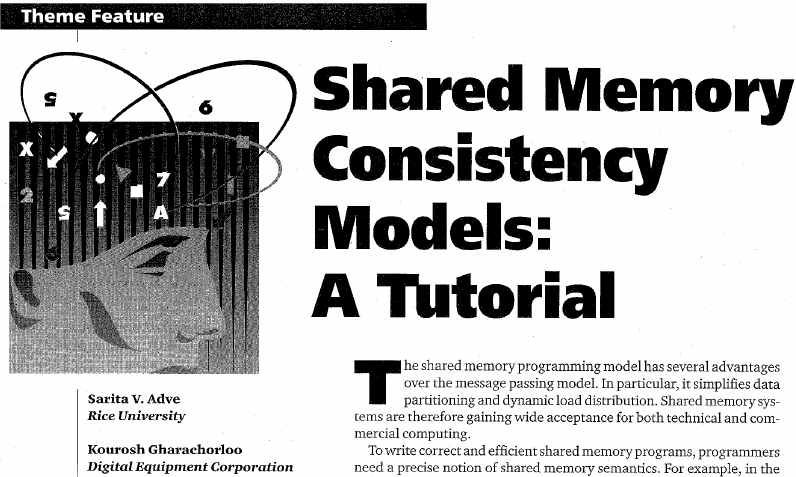
\includegraphics[width = 0.80\textwidth]{figures/ieee-computer-tutorial.png}
	  \caption{Tutorial \citeinbeamer{Adve}{IEEE Computer}{96}.}
	\end{subfigure}
  \end{figure}
\end{frame}
%%%%%%%%%%%%%%%
\begin{frame}{多处理器系统领域中的数据一致性理论}
  \answer{特性: ``以程序为导向、强调正确性''}
  \vspace{0.20cm}

  ``相对于 SC {\small (Sequential Consistency)}''的正确性~\footnote{术语称为 SCNF: Sequential Consistency Normal Form.} \citeinbeamer{Adve}{ISCA}{90}:

  \begin{columns}
	\column{0.60\textwidth}
	  \begin{description}
		\item[一致性:] 一致性模型 + \textcolor{red}{编程模型}
		\item[程序:] 遵循预定规则
		\item[系统:] 提供 SC 保证
		\item<3>[权衡:] 易编程性 vs. 性能
	  \end{description}
	\column{0.35\textwidth}
	\uncover<2->{\fignocaption{width = 0.50\textwidth}{figures/jsr133-jmm.png}}
  \end{columns}

  % \fig{width = 0.35\textwidth}{figures/consistency-lattice.png}{一致性模型 {\scriptsize (依据 \citeinbeamer{Steinke}{JACM}{04} 中 Figure~13 重绘)}.}
\end{frame}
%%%%%%%%%%%%%%%
\begin{frame}{分布式系统领域中的数据一致性理论}
  分布数据一致性问题是分布式系统设计的核心问题之一:
  \vspace{0.50cm}

  \begin{figure}
	\begin{subfigure}{0.48\textwidth}
	  \centering
	  \includegraphics[width = 0.90\textwidth]{figures/bayou-paper.png}
	  \caption{Eventual Consistency \citeinbeamer{Terry}{SOSP}{95}.}
	\end{subfigure}%
	\begin{subfigure}{0.48\textwidth}
	  \centering
	  \includegraphics[width = 0.85\textwidth]{figures/dsss.pdf}
	  \caption{分布式存储系统 {\tiny (\textcolor{blue}{左: 开源}; \textcolor{red}{右: 商用})}.} % (\textcolor{blue}{\scriptsize 开源 [左]} \& \textcolor{red}{\scriptsize 商用 [右]})
	\end{subfigure}
  \end{figure}
\end{frame}
%%%%%%%%%%%%%%%
% \begin{frame}{数据一致性问题研究的历史阶段}
%   \fignocaption{width = 0.90\textwidth}{figures/consistency-model-history.pdf}
% 
% \end{frame}
%%%%%%%%%%%%%%%
\begin{frame}{分布式系统领域中的数据一致性理论}
  \answer{更复杂的权衡\only<1-2>{:} \uncover<3->{$\Longrightarrow$ 一致性理论不追求``相对于 SC''的正确性}}

  \fignocaption{width = 0.30\textwidth}{figures/consistency-centric-tradeoff.pdf}
  \vspace{-0.80cm}

  \uncover<2->{
  \begin{columns}
	\column{0.45\textwidth}
	  \fig{width = 0.50\textwidth}{figures/cap-theorem.png}{CAP 定理 \citeinbeamer{Brewer}{PODC}{00}}
	\column{0.50\textwidth}
	  \fig{width = 0.65\textwidth}{figures/pacelc-tradeoff-new.pdf}{PACELC 权衡 \citeinbeamer{Abadi}{IEEE Computer}{12}}
  \end{columns}
  }
\end{frame}
%%%%%%%%%%%%%%%
\begin{frame}{分布式系统领域中的数据一致性理论}
  \answer{更丰富的应用\only<1>{:} \uncover<2>{$\Longrightarrow$ 一致性理论应体现应用的多样性}}
  \vspace{0.50cm}

  \begin{columns}
	\column{0.45\textwidth}
	  \fig{width = 0.75\textwidth}{figures/cassandra-and-datastax.jpg}{Cassandra 分布式存储系统.}
	\column{0.45\textwidth}
	  \fig{width = 0.90\textwidth}{figures/cassandra-datastax-customers.png}{Cassandra \& DataStax 客户.}
  \end{columns}
\end{frame}
%%%%%%%%%%%%%%%
% \begin{frame}{分布式系统领域数据一致性理论}
%   \graphicspath{{tikz-in-beamer/}}
%   \begin{figure}[h!]
%     \centering
%     \begin{adjustbox}{max totalsize = {1.00\textwidth}{1.00\textheight}, center}
% 	  %%%%% Description: beamer overlay for history of (weak) consistency models in the context of distributed systems. %%%%%
%%%%% Date: July 25, 2016 %%%%%
%%%%% Author: Hengfeng Wei (hengxin) %%%%

\begin{tikzpicture}[comment/.style = {align = center},
	axis/.style = {dashed, dash pattern = on 8pt off 4pt, line width = 2pt, draw = red},
	sepline/.style = {dashed, line width = 2pt, opacity = 0.80, blue},
    node distance = 2.0cm]

  %%%%%%%%%% Begin: years and papers %%%%%%%%%% 
  % \x: x coordinate; \y: year; \n: name; \lbl: label
  \foreach \x/\y/\n/\lbl in {
	1/1995/eventual/\textcolor{blue}{Eventual consistency},
	6/2000/cap/\textcolor{red}{\bf CAP theorem},
	12/2006/bigtable/\textcolor{blue}{Bigtable@Google},
	18/2007/dynamo/\textcolor{blue}{Dynamo@Amazon},
	25/2012/pacelc/\textcolor{red}{\bf PACELC tradeoff}} {
	\node[star, star points = 5, minimum size = 3pt, draw = red, fill = yellow, line width = 2pt] (\x) at (\x, 5) {};
	\node[below = 0.50cm of \x, font = \large] (\y) {\bf \y};
	\node[above = 0.50cm of \x, align = center, font = \Large] (\n) {\lbl};
  }

  \path[axis] (1) to (6) to (12) to (18) to (25);
  \draw[> = stealth, ->, axis] (25) to (27, 5);
  %%%%%%%%%% End: decades and systems %%%%%%%%%% 
  \draw[sepline] (8, 1) to (8, 10);
  \draw[sepline] (22, 1) to (22, 10);

  \pause
  %%%%% bayou system %%%%%
  \node[below = of 1995] (bayou-fig) {\includegraphics[scale = 0.35]{figs/bayou-paper.png}};
  \node[above = of eventual] (bayou-eventual) {
\includegraphics[scale = 0.13]{figs/24-7-service.png}};

  %%%%% cap theorem %%%%%
  \node[below = of 2000] (cap-ppt) {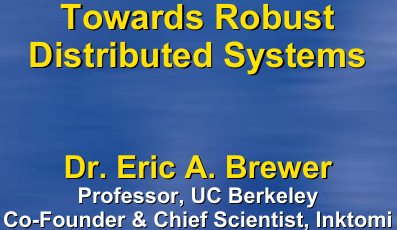
\includegraphics[scale = 0.35]{figs/cap-keynote-ppt.png}};
  % \node[above = of cap] (cap-fig) {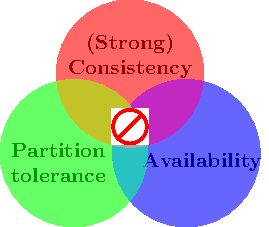
\includegraphics[scale = 0.90]{cap-theorem.pdf}}; 
  \node[above = of cap] (cap-fig) {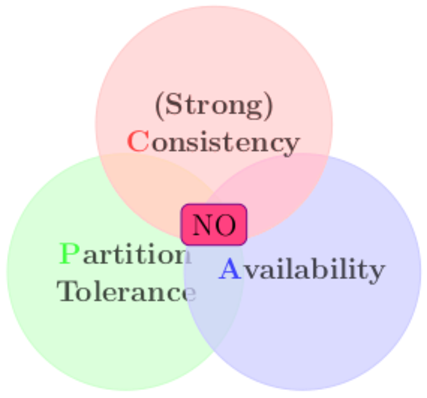
\includegraphics[scale = 0.55]{figs/cap-theorem-no-text.pdf}}; 

  \pause
  %%%%% bigtable %%%%%
  \node[below = of 2006, opacity = 0.80] (bigtable-fig) {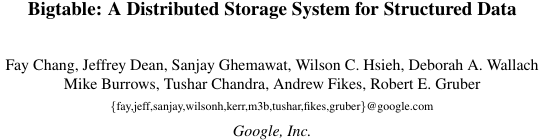
\includegraphics[scale = 0.50]{figs/bigtable-paper.png}};
  \node[above = of bigtable] (bigtable-tradeoff) {
\includegraphics[scale = 0.10]{figs/unavailable.png}};
  
  \pause
  %%%%% dynamo %%%%%
  \node[below = of 2007, opacity = 0.70] (dynamo-fig) {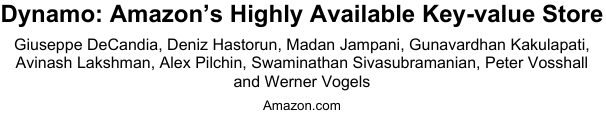
\includegraphics[scale = 0.50]{figs/dynamo-paper.png}};
  \node[above = of dynamo] (dynamo-tradeoff) {
\includegraphics[scale = 0.06]{figs/eventually.jpg}};

  \pause
  %%%%% more systems %%%%%
  \node[] (systems) at ($0.50*(bigtable) + 0.50*(dynamo) + (0, -0.50cm)$) {\includegraphics[scale = 0.80]{figs/dsss.pdf}};

  \pause
  %%%%% pacelc tradeoff %%%%%
  \node[below = of 2012] (pacelc-paper) {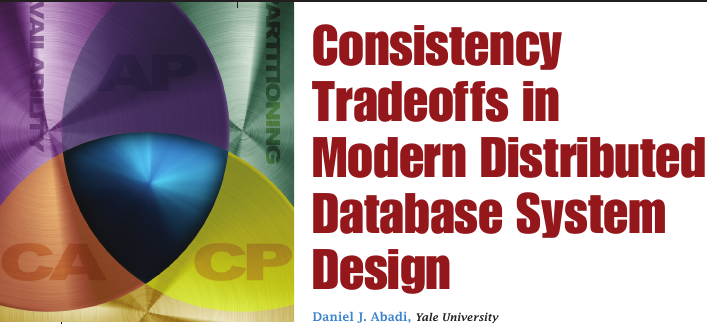
\includegraphics[scale = 0.25]{figs/pacelc-paper.png}};
  \node[above = of pacelc] (pacelc-fig) {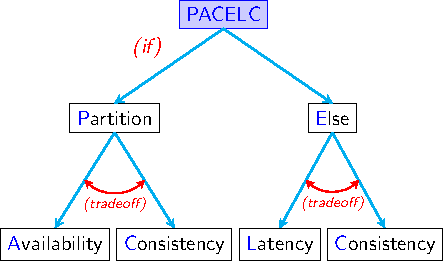
\includegraphics[scale = 0.80]{figs/pacelc-tradeoff-new.pdf}};
\end{tikzpicture}

%     \end{adjustbox}
%   \end{figure}
% \end{frame}
%%%%%%%%%%%%%%%
% \begin{frame}{数据一致性问题研究的历史阶段 (结论)}
%   \begin{columns}[T]
% 	\column{0.40\textwidth}
% 	  新平台, 新特点:
% 	  \vspace{0.30cm}
% 	  \begin{itemize}
% 		\item 更丰富的应用
% 		\item 更复杂的权衡
% 	  \end{itemize}
% 	\column{0.45\textwidth}
% 	\only<2->{更具\textcolor{brown}{``柔性''}的数据一致性理论:}
% 	  \vspace{0.30cm}
% 	  \begin{itemize}
% 		\item<3-> 多样化, 可调节
% 		\item<4-> 精细化, 可度量
% 	  \end{itemize}
%   \end{columns}
% \end{frame}

  % \uncover<1->{\textcolor{blue}{需要什么样的数据一致性理论?}}
  % \vspace{0.30cm}

  % \begin{columns}[t]
  %   \column{0.50\textwidth}
  %     \uncover<2->{
  %     (1) 
  %     } 
  %   \column{0.50\textwidth}
  %     \uncover<3->{
  %    (2) 体现更丰富的 tradeoffs
  %     \fignocaption{width = 0.60\textwidth}{figures/consistency-centric-tradeoff.pdf}
  %     }
  % \end{columns}
%%%%%%%%%%%%%%%
\begin{frame}{分布数据一致性问题研究理念 (I)}
  % \begin{center}
  %   \textcolor{red}{新平台, 新特点:} 更复杂的权衡、更丰富的应用
  % \end{center}
  \textcolor{red}{新平台, 新特点:} 

  \begin{itemize}
	\item<2-> 更复杂的权衡 $\Longrightarrow$ 正确性变得模糊
	\item<3-> 更丰富的应用 $\Longrightarrow$ 多样性变得重要
  \end{itemize}

  % \vspace{0.50cm}
  % \only<2>{
  % 棒球赛应用一致性需求~\citeinbeamer{Terry}{SOSP}{13}:
  % \begin{description}
  %   \item[记分员:] 采用 \textcolor{blue}{\texttt{\small read-my-writes consistency}} 更新比赛得分
  %   \item[电台记者:] 采用 \textcolor{blue}{\texttt{\small monotonic reads consistency}} 避免读到陈旧比分
  % \end{description}
  % }

  % \vspace{0.25cm}
  % \only<3>{
  % 出租车实时位置查询一致性需求:
  % \begin{description}
  %   \item[权衡:] 为了保证低延迟, 允许违反 \textcolor{blue}{\texttt{\small atomicity}}
  %   \item[有界:] 所有读请求都要满足 \textcolor{blue}{\texttt{\small 2-atomicity}}
  %   \item[量化需求:] 违反 \textcolor{blue}{\texttt{\small atomicity}} 的读请求低于$1\%$ 
  % \end{description}
  % }

  \vspace{1.00cm}
  \uncover<4->{
	\centerline{需要更具\textcolor{brown}{``柔性''}的分布数据一致性理论:}
  }
  \begin{description}
	\centering
	\item<5>[理念一:] 多样化, 可调节
	\item<5>[理念二:] 精细化, 可度量
  \end{description}
\end{frame}
%%%%%%%%%%%%%%%
\begin{frame}{数据一致性问题研究理念 (II)}
  \begin{description}
	\setlength{\itemsep}{10pt}
	\item[多样化:] 从单一到融合 (mono- vs. multi-) \citeinbeamer{Terry}{CACM}{13} 
	  \vspace{5pt}
	  \begin{itemize}
		\setlength{\itemsep}{5pt}
		\item 融合强弱一致性: 不同操作, 不同一致性需求 
		\item 融合一致与不一致: 容忍``有限度''的不一致
	  \end{itemize}
	  \begin{columns}
		\column{0.50\textwidth}
		  \fignocaption{width = 0.50\textwidth}{figures/tradeoff.jpg} 
		\column{0.50\textwidth}
		  \fignocaption{width = 0.35\textwidth}{figures/one-size-fit-all-text.jpg} 
	  \end{columns}
	\pause
	\item[可调节:] think \textcolor{red}{\it dynamically} \citeinbeamer{Terry}{SOSP}{13}
	  \vspace{10pt}
	  \begin{center}
	    依据应用需求/系统状态调节数据一致性
	  \end{center}
  \end{description}
\end{frame}
%%%%%%%%%%%%%%%
\begin{frame}{数据一致性问题研究理念 (III)}
  \begin{description}
	\setlength{\itemsep}{20pt}
	\item[精细化:] 从二元 {\small \;$\set{0,1}$} 到连续谱 {\small \;$(0,1)$}~\citeinbeamer{Yu}{TOCS}{02}
	  \begin{columns}
		\column{0.50\textwidth}
		  \fignocaption{scale = 0.15}{figures/black-or-white.jpg}
		\column{0.50\textwidth}
		  \fignocaption{scale = 0.05}{figures/prism-spectrum.jpg}
	  \end{columns}
	  \pause
	\item[可度量:] think \textcolor{red}{\it probabilistically} \citeinbeamer{Brewer}{PODC}{00}
	  \vspace{10pt}
	  \begin{center}
		度量系统/系统执行对一致性的满足程度
	  \end{center}
  \end{description}
\end{frame}
%%%%%%%%%%%%%%%
\begin{frame}{数据一致性问题研究理念 (IV)}
  \mdf{red}{red}{论文研究问题}{teal}{如何在分布式系统中\\落实\idea{}的\\分布数据一致性问题研究理念?}

  \pause

  \mdf{blue}{blue}{论文主要贡献}{black}{
	\begin{description}
	  \item<2->[理念:] 提出\idea{}的数据\\一致性问题研究理念
	  \item<+->[框架:] 提出包含``一个基础、三个维度''的技术框架 
	  \item<+->[VPC:] 验证 Pipelined-RAM Consistency \hfill \textcolor{brown}{\scriptsize [``精细化, 可度量'']}
	  \item<.->[PA2AM:]	量化 2-Atomicity 协议 \hfill \textcolor{brown}{\scriptsize [``精细化, 可度量'']} 
	  \item<.->[RVSI:] 可调节 Snapshot Isolation \hfill \textcolor{brown}{\scriptsize [``多样化, 可调节'']}
	\end{description}
  }
\end{frame}
%%%%%%%%%%%%%%%
% \section{相关工作}	\label{section:related-work}

% \includeonlyframes{related-work-categories,related-work-summary}
% 
% %%%%%%%%%%%%%%%
\begin{frame}[label = related-work-categories]{相关工作分类}
  \begin{table}[]
	\centering
	\caption{\idea{}研究理念相关工作.}
	\renewcommand\arraystretch{2}
	\resizebox{\textwidth}{!}{%
	  \begin{tabular}{cc|c|c|c|c|}
		\cline{3-6}
		\multicolumn{2}{c|}{} & \multicolumn{2}{c|}{\textbf{读写寄存器}} & \multicolumn{2}{c|}{\textbf{事务}} \\ \cline{3-6}
		\multicolumn{2}{c|}{} & 多处理器系统 & 分布式系统 & \only<1>{多处理器系统}\only<2>{\textcolor{gray}{多处理器系统}} & 分布式系统 \\ \hline
		\multicolumn{2}{|c|}{\textbf{\ideadt{}}} &  &  
		& \uncover<2>{\multirow{3}{*}{\begin{tabular}[c]{@{}c@{}}\textcolor{gray}{软件}\\ \textcolor{gray}{事务内存}\end{tabular}}} &  
		% \\ \hline
		\\ \cline{1-4} \cline{6-6}
		\multicolumn{1}{|c|}{\multirow{2}{*}{\textbf{\idearm{}}}} & 验证 &  &  &  &  
		% \\ \cline{2-6}
		\\ \cline{2-4} \cline{6-6}
		\multicolumn{1}{|c|}{} & 量化 &  &  &  &  
		\\ \hline
	  \end{tabular}
    }
  \end{table}
\end{frame}
%%%%%%%%%%%%%%%
\begin{frame}{\ideadt{}的研究理念 (一)}
  \begin{table}[]
	\centering
	\renewcommand\arraystretch{1.5}
	\resizebox{\textwidth}{!}{%
	  \begin{tabular}{cc|c|c|c|c|}
		\cline{3-6}
		\multicolumn{2}{c|}{} & \multicolumn{2}{c|}{\textbf{读写寄存器}} & \multicolumn{2}{c|}{\textbf{事务}} \\ \cline{3-6} 
		\multicolumn{2}{c|}{} & 多处理器系统 & 分布式系统 & 多处理器系统 & 分布式系统 \\ \hline
		\multicolumn{2}{|c|}{\textbf{\ideadt{}}} & \only<1-3>{\textcolor{red}{\bf \checkmark}} 
		\only<4->{\begin{tabular}[c]{@{}c@{}}\textcolor{red}{相关工作丰富}\\ \textcolor{red}{理论扎实}\end{tabular}} &  &  &  \\ \hline
	  \end{tabular}%
	}
  \end{table}

  \pause 

  \begin{description}
	\setlength{\itemsep}{5pt}
	\item[典型:] Hybrid consistency \citeinbeamer{Attiya}{SICOMP}{98}
	\item[思想:] 将操作分为强弱两类
	  \pause
	\item[其它:] ``带同步的''一致性模型 \citeinbeamer{Dubois}{IEEE Computer}{88} \citeinbeamer{Steinke}{JACM}{04}
	\item[特点:] 强调正确性 {\footnotesize (properly synchronized)}
  \end{description}
\end{frame}
%%%%%%%%%%%%%%%
\begin{frame}{\ideadt{}的研究理念 (二)}
  \begin{table}[]
	\centering
	\renewcommand\arraystretch{1.5}
	\resizebox{\textwidth}{!}{%
	  \begin{tabular}{cc|c|c|c|c|}
		\cline{3-6}
		\multicolumn{2}{c|}{} & \multicolumn{2}{c|}{\textbf{读写寄存器}} & \multicolumn{2}{c|}{\textbf{事务}} \\ \cline{3-6} 
		\multicolumn{2}{c|}{} & 多处理器系统 & 分布式系统 & 多处理器系统 & 分布式系统 \\ \hline
		\multicolumn{2}{|c|}{\textbf{\ideadt{}}} & {\begin{tabular}[c]{@{}c@{}}{\small 相关工作丰富}\\ {\small 理论扎实}\end{tabular}}
		& \only<1-3>{\textcolor{red}{\bf \checkmark}} 
		\only<4->{\begin{tabular}[c]{@{}c@{}}\textcolor{red}{渐成趋势}\\ \textcolor{red}{理论欠缺}\end{tabular}} &  &  \\ \hline
	  \end{tabular}%
	}
  \end{table}

  \pause 

  \begin{description}
	\setlength{\itemsep}{5pt}
	\item[思想:] 借鉴并发展 Hybrid consistency 的思想
	\item[典型:] 
	  \begin{itemize}
		\item Causal+forced+immediate operations \citeinbeamer{Ladin}{TOCS}{92}
		\item RedBlue consistency \citeinbeamer{Li}{OSDI}{12}
		% \item Apache Cassandra~\footnote{\url{http://cassandra.apache.org/}} \citeinbeamer{Facebook}{SIGOPS OSR}{10}
		\item Pileus \citeinbeamer{Terry}{SOSP}{13}
	  \end{itemize}
	  \pause
	\item[特点:] 更细粒度的多一致性模型共存、更能容忍数据不一致
  \end{description}
\end{frame}
%%%%%%%%%%%%%%%
\begin{frame}{\ideadt{}的研究理念 (三)}
  \begin{table}[]
	\centering
	\renewcommand\arraystretch{1.5}
	\resizebox{\textwidth}{!}{%
	  \begin{tabular}{cc|c|c|c|c|}
		\cline{3-6}
		\multicolumn{2}{c|}{} & \multicolumn{2}{c|}{\textbf{读写寄存器}} & \multicolumn{2}{c|}{\textbf{事务}} \\ \cline{3-6} 
		\multicolumn{2}{c|}{} & 多处理器系统 & 分布式系统 & 多处理器系统 & 分布式系统 \\ \hline
		\multicolumn{2}{|c|}{\textbf{\ideadt{}}} & {\begin{tabular}[c]{@{}c@{}}{\small 相关工作丰富}\\ {\small 理论扎实}\end{tabular}}
		& \begin{tabular}[c]{@{}c@{}}{\small 渐成趋势}\\ {\small 理论欠缺}\end{tabular} 
		& \textcolor{gray}{\small 软件事务内存}
		& \only<1-2>{\textcolor{red}{\bf \checkmark}} 
		  \only<3->{\textcolor{red}{探索阶段}} \\ \hline
		  % \only<4->{\begin{tabular}[c]{@{}c@{}}\textcolor{red}{探索阶段}\\ \textcolor{red}{系统、理论欠缺}\end{tabular}} \\ \hline
	  \end{tabular}
	}
  \end{table}

  \begin{description}
	\setlength{\itemsep}{5pt}
	\item[思想:] 多个事务一致性模型共存
	\item[典型:] 
	  \begin{itemize}
		\item RC-SR {\scriptsize (relaxed currency serializability)} \citeinbeamer{Bernstein}{SIGMOD}{06}
		\item Pileus consistency choices \citeinbeamer{Terry}{MSR-TR}{13}
		\item Multi-level CSI {\scriptsize (Causal Snapshot Isolation)} \citeinbeamer{Tripathi}{BigData}{15}
	  \end{itemize}
	  \pause
	\item[挑战:] ``多样化''事务语义; 可扩展的系统实现
  \end{description}
\end{frame}
%%%%%%%%%%%%%%%
\begin{frame}{\idearm{}的研究理念 (一)}
  \begin{table}[]
	\centering
	\renewcommand\arraystretch{1.6}
	\resizebox{\textwidth}{!}{%
	  \begin{tabular}{cc|c|c|c|c|}
		\cline{3-6}
		\multicolumn{2}{c|}{} & \multicolumn{2}{c|}{\textbf{读写寄存器}} & \multicolumn{2}{c|}{\textbf{事务}} \\ \cline{3-6} 
		\multicolumn{2}{c|}{} & 多处理器系统 & 分布式系统 & 多处理器系统 & 分布式系统 \\ \hline
		\multicolumn{1}{|c|}{\only<1-2>{\multirow{2}{*}{\textbf{\idearm{}}}}\only<3>{\multirow{2}{*}[-0.5em]{\textbf{\idearm{}}}}\only<4->{\multirow{2}{*}[-1em]{\textbf{\idearm{}}}}} 
		& 验证 
		& \only<2>{\textcolor{red}{\bf \checkmark}}\only<3>{\begin{tabular}[c]{@{}c@{}}\textcolor{red}{典型模型}\\ \textcolor{red}{理论全面}\end{tabular}}\only<4>{\begin{tabular}[c]{@{}c@{}}{\small 典型模型}\\ {\small 理论全面}\end{tabular}} &  &  &  \\ \cline{2-6} 
		\multicolumn{1}{|c|}{} & 量化 & \only<4->{\begin{tabular}[c]{@{}c@{}}\textcolor{red}{暂无}\\ \textcolor{red}{强调正确性}\end{tabular}} &  &  &  \\ \hline
	  \end{tabular}
	}
  \end{table}

  \pause

  典型的一致性模型验证 \textcolor{blue}{\small (Verify)} 问题:
  \begin{itemize}
	\item VSC {\scriptsize (Sequential Consistency)}, VL {\scriptsize (Linearizability)} \citeinbeamer{Gibbons}{SICOMP}{97}
	\item VMC {\scriptsize (Memory Coherence)} \citeinbeamer{Cantin}{SPAA}{03} \citeinbeamer{Cantin}{TPDS}{05}
	\item VTSO {\scriptsize (Total Store Order)} \citeinbeamer{Hangal}{ISCA}{03} \citeinbeamer{Manovit}{SPAA}{05} 
	  \citeinbeamer{Roy}{CAV}{06} \citeinbeamer{Baswana}{CAV}{08}
  \end{itemize}
\end{frame}
%%%%%%%%%%%%%%%
\begin{frame}{\idearm{}的研究理念 (二)}
  \begin{table}[]
	\centering
	\renewcommand\arraystretch{1.6}
	\resizebox{\textwidth}{!}{%
	  \begin{tabular}{cc|c|c|c|c|}
		\cline{3-6}
		\multicolumn{2}{c|}{} & \multicolumn{2}{c|}{\textbf{读写寄存器}} & \multicolumn{2}{c|}{\textbf{事务}} \\ \cline{3-6} 
		\multicolumn{2}{c|}{} & 多处理器系统 & 分布式系统 & 多处理器系统 & 分布式系统 \\ \hline
		\multicolumn{1}{|c|}{\multirow{2}{*}[-1em]{\textbf{\idearm{}}}} & 验证 
		& \begin{tabular}[c]{@{}c@{}}{\small 典型模型}\\ {\small 理论全面}\end{tabular} 
		& \only<1-2>{\textcolor{red}{\bf \checkmark}}\only<3->{\begin{tabular}[c]{@{}c@{}}\textcolor{red}{弱模型验证}\\ \textcolor{red}{有待研究}\end{tabular}} &  &  \\ \cline{2-6} 
		\multicolumn{1}{|c|}{} & 量化 & \begin{tabular}[c]{@{}c@{}}{\small 暂无}\\ {\small 强调正确性}\end{tabular} &  &  &  \\ \hline
	  \end{tabular}
	}
  \end{table}

  \begin{description}
	\item[动机:] 商业条款 SLA {\scriptsize (Service Level Agreement)} \citeinbeamer{Amazon}{SOSP}{07}
	  \pause
	\item[特点:] 在线验证 safeness, regularity, atomicity \citeinbeamer{Golab}{PODC}{11}
	  \pause
	\item[不足:] 常用 Pipelined-RAM consistency, causal consistency, \\hybrid consistency 验证问题有待研究
  \end{description}
\end{frame}
%%%%%%%%%%%%%%%
\begin{frame}{\idearm{}的研究理念 (三)}
  \begin{table}[]
	\centering
	\renewcommand\arraystretch{1.6}
	\resizebox{\textwidth}{!}{%
	  \begin{tabular}{cc|c|c|c|c|}
		\cline{3-6}
		\multicolumn{2}{c|}{} & \multicolumn{2}{c|}{\textbf{读写寄存器}} & \multicolumn{2}{c|}{\textbf{事务}} \\ \cline{3-6} 
		\multicolumn{2}{c|}{} & 多处理器系统 & 分布式系统 & 多处理器系统 & 分布式系统 \\ \hline
		\multicolumn{1}{|c|}{\multirow{2}{*}[-1em]{\textbf{\idearm{}}}} & 验证 
		& \begin{tabular}[c]{@{}c@{}}{\small 典型模型}\\ {\small 理论全面}\end{tabular} 
		& \begin{tabular}[c]{@{}c@{}}{\small 弱模型验证}\\ {\small 有待研究}\end{tabular} 
		&  &  \\ \cline{2-6} 
		\multicolumn{1}{|c|}{} & 量化 
		& \begin{tabular}[c]{@{}c@{}}{\small 暂无}\\ {\small 强调正确性}\end{tabular}
		& \only<2>{\textcolor{red}{\bf \checkmark}}\only<3>{\begin{tabular}[c]{@{}c@{}}\textcolor{red}{量化执行易}\\ \textcolor{red}{量化协议难}\end{tabular}}
		&  &  \\ \hline
	  \end{tabular}
	}
  \end{table}

  \pause

  \begin{description}
	\item[量化执行:] $k$/$\Delta$/$\Gamma$-atomicity {\tiny{\textcolor{blue}{[Golab@PODC'11, ICDCS'13, ICDCS'14, PODC'15]}}}
	\item[量化协议:] probabilistic regularity/atomicity \\ \citeinbeamer{Yu}{DISC}{03} \citeinbeamer{Lee}{DC}{05} \citeinbeamer{Gramoli}{OPODIS}{07} \citeinbeamer{Bailis}{PVLDB}{12}
  \end{description}
\end{frame}
%%%%%%%%%%%%%%%
\begin{frame}{\idearm{}的研究理念 (四)}
  \begin{table}[]
	\centering
	\renewcommand\arraystretch{1.6}
	\resizebox{\textwidth}{!}{%
	  \begin{tabular}{cc|c|c|c|c|}
		\cline{3-6}
		\multicolumn{2}{c|}{} & \multicolumn{2}{c|}{\textbf{读写寄存器}} & \multicolumn{2}{c|}{\textbf{事务}} \\ \cline{3-6} 
		\multicolumn{2}{c|}{} & 多处理器系统 & 分布式系统 & \textcolor{gray}{多处理器系统} & 分布式系统 \\ \hline
		\multicolumn{1}{|c|}{\multirow{2}{*}[-1em]{\textbf{\idearm{}}}} & 验证 
		& \begin{tabular}[c]{@{}c@{}}{\small 典型模型}\\ {\small 理论全面}\end{tabular} 
		& \begin{tabular}[c]{@{}c@{}}{\small 弱模型验证}\\ {\small 有待研究}\end{tabular} 
		& \multirow{2}{*}[-1em]{\begin{tabular}[c]{@{}c@{}}\textcolor{gray}{\small 软件事务内存}\end{tabular}}
		& \only<1-2>{\textcolor{red}{\bf \checkmark}}\only<3->{\begin{tabular}[c]{@{}c@{}}\textcolor{red}{理论全面}\\ \textcolor{red}{指导协议设计}\end{tabular}}
		\\ \cline{2-4} \cline{6-6}
		\multicolumn{1}{|c|}{} & 量化 
		& \begin{tabular}[c]{@{}c@{}}{\small 暂无}\\ {\small 强调正确性}\end{tabular}
		& \begin{tabular}[c]{@{}c@{}}{\small 量化执行易}\\ {\small 量化协议难}\end{tabular}
		&  &  \\ \hline
	  \end{tabular}
	}
  \end{table}

  \begin{itemize}
	\item SR {\scriptsize (Serializability)} 强一致性模型及变体  
	  \\ \citeinbeamer{Papadimitriou}{JACM}{79} \citeinbeamer{Bernstein}{TODS}{83} \citeinbeamer{Yannakakis}{JACM}{84} 
	\item SI {\scriptsize (Snapshot Isolation)} 等弱一致性模型 
	  \\ \citeinbeamer{Adya}{Phd-Thesis}{99} \citeinbeamer{Fekete}{TODS}{05} \citeinbeamer{Cahill}{SIGMOD}{08} \citeinbeamer{Zellag}{VLDB}{14}
  \end{itemize}
\end{frame}
%%%%%%%%%%%%%%%
\begin{frame}{\idearm{}的研究理念 (五)}
  \begin{table}[]
	\centering
	\renewcommand\arraystretch{1.6}
	\resizebox{\textwidth}{!}{%
	  \begin{tabular}{cc|c|c|c|c|}
		\cline{3-6}
		\multicolumn{2}{c|}{} & \multicolumn{2}{c|}{\textbf{读写寄存器}} & \multicolumn{2}{c|}{\textbf{事务}} \\ \cline{3-6} 
		\multicolumn{2}{c|}{} & 多处理器系统 & 分布式系统 & \textcolor{gray}{多处理器系统} & 分布式系统 \\ \hline
		\multicolumn{1}{|c|}{\multirow{2}{*}[-1em]{\textbf{\idearm{}}}} & 验证 
		& \begin{tabular}[c]{@{}c@{}}{\small 典型模型}\\ {\small 理论全面}\end{tabular} 
		& \begin{tabular}[c]{@{}c@{}}{\small 弱模型验证}\\ {\small 有待研究}\end{tabular} 
		& \multirow{2}{*}[-1em]{\begin{tabular}[c]{@{}c@{}}\textcolor{gray}{\small 软件事务内存}\end{tabular}}
		& \begin{tabular}[c]{@{}c@{}}{\small 理论全面}\\ {\small 指导协议设计}\end{tabular}
		\\ \cline{2-4} \cline{6-6}
		\multicolumn{1}{|c|}{} & 量化 
		& \begin{tabular}[c]{@{}c@{}}{\small 暂无}\\ {\small 强调正确性}\end{tabular}
		& \begin{tabular}[c]{@{}c@{}}{\small 量化执行易}\\ {\small 量化协议难}\end{tabular}
		&  
		& \begin{tabular}[c]{@{}c@{}}\textcolor{red}{量化协议难}\\ \textcolor{red}{相关工作少}\end{tabular} 
		\\ \hline
	  \end{tabular}
	}
  \end{table}

  \begin{itemize}
	\item 量化 SI {\scriptsize (Snapsho Isolation)} 与 RC {\scriptsize (Read Committed)} 协议 \citeinbeamer{Fekete}{PVLDB}{09}
  \end{itemize}
\end{frame}
%%%%%%%%%%%%%%%
\begin{frame}[label = related-work-summary]{相关工作总结}
  \begin{table}[]
	\centering
	\caption{\idea{}研究理念相关工作.}
	\renewcommand\arraystretch{1.6}
	\resizebox{\textwidth}{!}{%
	  \begin{tabular}{cc|c|c|c|c|}
		\cline{3-6}
		\multicolumn{2}{c|}{} & \multicolumn{2}{c|}{\textbf{读写寄存器}} & \multicolumn{2}{c|}{\textbf{事务}} \\ \cline{3-6} 
		\multicolumn{2}{c|}{} & 多处理器系统 & \cellcolor{red!80}{分布式系统} & \textcolor{gray}{多处理器系统} & \cellcolor{red!80}{分布式系统} \\ \hline

		\multicolumn{2}{|c|}{\textbf{\ideadt{}}} & {\begin{tabular}[c]{@{}c@{}}{\small 相关工作丰富}\\ {\small 理论扎实}\end{tabular}}
		& \begin{tabular}[c]{@{}c@{}}{\small 渐成趋势}\\ {\small 理论欠缺}\end{tabular} 
		& \multirow{2}{*}[-3em]{\begin{tabular}[c]{@{}c@{}}\textcolor{gray}{\small 软件}\\ \textcolor{gray}{\small 事务内存}\end{tabular}}
		& \cellcolor{brown!80}{\small 探索阶段} \\ \cline{1-4} \cline{6-6}

		\multicolumn{1}{|c|}{\multirow{2}{*}[-1em]{\textbf{\idearm{}}}} & 验证 
		& \begin{tabular}[c]{@{}c@{}}{\small 典型模型}\\ {\small 理论全面}\end{tabular} 
		& \cellcolor{brown!80}{\begin{tabular}[c]{@{}c@{}}{\small 弱模型验证}\\ {\small 有待研究}\end{tabular}}
		& 
		& \begin{tabular}[c]{@{}c@{}}{\small 理论全面}\\ {\small 指导协议设计}\end{tabular}
		\\ \cline{2-4} \cline{6-6} \hhline{*{3}{~}-*{2}{~}}

		\multicolumn{1}{|c|}{} & 量化 
		& \begin{tabular}[c]{@{}c@{}}{\small 暂无}\\ {\small 强调正确性}\end{tabular}
		& \cellcolor{brown!80}{\begin{tabular}[c]{@{}c@{}}{\small 量化执行易}\\ {\small 量化协议难}\end{tabular}}
		&  
		& \begin{tabular}[c]{@{}c@{}}{\small 量化协议难}\\ {\small 相关工作少}\end{tabular} 
		\\ \hline
	  \end{tabular}
	}
  \end{table}
\end{frame}
%%%%%%%%%%%%%%%

%%%%%%%%%%%%%%%
\begin{frame}{相关工作分类}
  \begin{table}[]
	\centering
	\caption{\idea{}研究理念相关工作.}
	\renewcommand\arraystretch{2}
	\resizebox{\textwidth}{!}{%
	  \begin{tabular}{cc|c|c|c|c|}
		\cline{3-6}
		\multicolumn{2}{c|}{} & \multicolumn{2}{c|}{\textbf{读写寄存器}} & \multicolumn{2}{c|}{\textbf{事务}} \\ \cline{3-6}
		\multicolumn{2}{c|}{} & 多处理器系统 & 分布式系统 & \textcolor{gray}{多处理器系统} & 分布式系统 \\ \hline
		\multicolumn{2}{|c|}{\textbf{\ideadt{}}} &  &  
		& \multirow{3}{*}{\begin{tabular}[c]{@{}c@{}}\textcolor{gray}{软件}\\ \textcolor{gray}{事务内存}\end{tabular}} &  
		% \\ \hline
		\\ \cline{1-4} \cline{6-6}
		\multicolumn{1}{|c|}{\multirow{2}{*}{\textbf{\idearm{}}}} & 验证 &  &  &  &  
		% \\ \cline{2-6}
		\\ \cline{2-4} \cline{6-6}
		\multicolumn{1}{|c|}{} & 量化 &  &  &  &  
		\\ \hline
	  \end{tabular}
    }
  \end{table}
\end{frame}
%%%%%%%%%%%%%%%
\begin{frame}{相关工作总结}
  \begin{table}[]
	\centering
	\caption{\idea{}研究理念相关工作.\protected\\(\hyperlink{appendix}{\textcolor{teal}{详见附录}})}
	\renewcommand\arraystretch{1.6}
	\resizebox{\textwidth}{!}{%
	  \begin{tabular}{cc|c|c|c|c|}
		\cline{3-6}
		\multicolumn{2}{c|}{} & \multicolumn{2}{c|}{\textbf{读写寄存器}} & \multicolumn{2}{c|}{\textbf{事务}} \\ \cline{3-6} 
		\multicolumn{2}{c|}{} & 多处理器系统 & \only<1>{分布式系统}\only<2->{\cellcolor{red}{分布式系统}} 
			& \textcolor{gray}{多处理器系统} & \only<1>{分布式系统}\only<2->{\cellcolor{red}{分布式系统}} \\ \hline

			\multicolumn{2}{|c|}{\only<1-2>{\bf \ideadt{}}\only<3->{\cellcolor{brown}{\bf \ideadt{}}}} 
			  & {\begin{tabular}[c]{@{}c@{}}{\small 相关工作丰富}\\ {\small 理论扎实}\end{tabular}}
		& \begin{tabular}[c]{@{}c@{}}{\small 渐成趋势}\\ {\small 理论欠缺}\end{tabular} 
		& \multirow{2}{*}[-3em]{\begin{tabular}[c]{@{}c@{}}\textcolor{gray}{\small 软件}\\ \textcolor{gray}{\small 事务内存}\end{tabular}}
		& {\small 探索阶段} \\ \cline{1-4} \cline{6-6}

		\multicolumn{1}{|c|}{\multirow{2}{*}[-1em]{\bf \idearm{}}}
		& \only<1-2>{验证}\only<3->{\cellcolor{brown}{验证}}
		& \begin{tabular}[c]{@{}c@{}}{\small 典型模型}\\ {\small 理论全面}\end{tabular} 
		& \begin{tabular}[c]{@{}c@{}}{\small 弱模型验证}\\ {\small 有待研究}\end{tabular}
		& 
		& \begin{tabular}[c]{@{}c@{}}{\small 理论全面}\\ {\small 指导协议设计}\end{tabular}
		\\ \cline{2-4} \cline{6-6}

		\multicolumn{1}{|c|}{} 
		& \only<1-3>{量化}\only<4->{\cellcolor{cyan}{量化}}
		& \begin{tabular}[c]{@{}c@{}}{\small 暂无}\\ {\small 强调正确性}\end{tabular}
		& \begin{tabular}[c]{@{}c@{}}{\small 量化执行易}\\ {\small 量化协议难}\end{tabular}
		&  
		& \begin{tabular}[c]{@{}c@{}}{\small 量化协议难}\\ {\small 相关工作少}\end{tabular} 
		\\ \hline
	  \end{tabular}
	}
  \end{table}

  \centerline{\uncover<2->{\textcolor{red}{1. 渐成趋势}} \qquad\quad
  \uncover<3->{\textcolor{brown}{2. 可资借鉴}} \qquad\quad
  \uncover<4->{\textcolor{cyan}{3. 问题凸显}}}
\end{frame}
%%%%%%%%%%%%%%%

% \section{技术框架}

\begin{comment}
%%%%%%%%%%%%%%%%%%%%%%%%%%%%%%
\subsection{理论模型:分布共享数据服务}

%%%%%%%%%%%%%%%
\begin{frame}{分布共享数据服务}
  \begin{columns}
	\column{0.50\textwidth}
	  \fignocaption{width = 0.60\textwidth}{figures/shared-data-clients.pdf}
	  \begin{center}
		共享数据系统
	  \end{center}
	\pause
	\column{0.50\textwidth}
	  \fignocaption{width = 0.70\textwidth}{figures/distributed-data-clients.pdf}
	  \begin{center}
		分布数据系统
	  \end{center}
  \end{columns}
\end{frame}
%%%%%%%%%%%%%%%
\begin{frame}{分布共享数据服务}
  \fignocaption{width = 0.45\textwidth}{figures/distributed-shared-data-clients.pdf}
  \begin{center}
	分布共享数据服务作为中间件管理分布数据
  \end{center}
\end{frame}
%%%%%%%%%%%%%%%
\begin{frame}{分布共享数据服务}
  \fignocaption{width = 0.35\textwidth}{figures/dsds.pdf}
  \begin{center}
	\textcolor{blue!80}{分布共享数据服务 \term{中间件}:} 在分布数据之上提供共享数据的抽象
  \end{center}
\end{frame}
%%%%%%%%%%%%%%%
\begin{frame}{分布共享数据服务 (注)}
  \begin{center}
	分布共享内存模型 (多处理器系统)\\
	\textcolor{blue}{[传统概念]}\\
	\vspace{0.10cm} +\\ \vspace{0.10cm}
	分布数据系统\\
	\textcolor{blue}{[新平台]}
	
	\uncover<2->{
	  \vspace{0.3cm}
	\color{red}\rule{0.618\linewidth}{3pt}
	  \vspace{0.2cm}

	\begin{center}
	  \textcolor{blue}{新平台凸显应用价值观:}
	  \begin{enumerate}
		\centering
		\item 多样化, 可调节
		\item 精细化, 可度量
	  \end{enumerate}
	\end{center}
	}
  \end{center}
\end{frame}
%%%%%%%%%%%%%%%
%%%%%%%%%%%%%%%%%%%%%%%%%%%%%%
\subsection{技术框架}
\end{comment}

%%%%%%%%%%%%%%%
\begin{frame}{分布数据一致性问题}
  \fignocaption{width = 0.618\textwidth}{figures/distributed-data-consistency-explained.pdf}
\end{frame}

% 分布数据一致性问题:
% \begin{itemize}
%   \item [\textcolor{blue}{\bf \cmark}] 分布: 分区 + 副本
%   \item [\textcolor{red}{\bf \xmark}] 数据: 数据类型
%   \item [\textcolor{red}{\bf \xmark}] 一致性: 关键问题
% \end{itemize}

% \textcolor{blue}{数据类型:}
% \begin{itemize}
%   \item 读写寄存器/变量 \textcolor{cyan}{\small ($x,y$)}
%   \item 数据结构 \textcolor{cyan}{\small (\textsc{Set, List})}
%   \item 事务 \textcolor{cyan}{\small (\textsc{Tx})}
% \end{itemize}

% \textcolor{blue}{一致性关键问题:}
% \begin{itemize}
%   \item 模型 \textcolor{cyan}{\small (semantics; 是什么)}
%   \item 机制 \textcolor{cyan}{\small (mechanism; 怎么做)}
%   \item 度量 \textcolor{cyan}{\small (measurement; 怎么样)}
% \end{itemize}
%%%%%%%%%%%%%%%
\begin{frame}{技术框架}
  \fig{width = 0.50\textwidth}{figures/3d-framework.pdf}{``一个基础, 三个维度''技术框架.}
\end{frame}
%%%%%%%%%%%%%%%
\begin{frame}{基础: 数据类型}
	数据类型: 从个体到群组
	\pause
	\vspace{0.20cm}
	\begin{itemize}
	  \setlength{\itemsep}{8pt}
	  \item<2-> 读写寄存器
	  \item<3-> 事务对象
		\begin{itemize}
		  \setlength{\itemsep}{4pt}
		  \item 事务 $\triangleq$ 多个读写寄存器的操作序列
		  \item 支持 ``all-or-none'' 语义
		  \item 易于开发并发应用
		\end{itemize}
	\end{itemize}
\end{frame}
%%%%%%%%%%%%%%%
\begin{frame}{维度一: 一致性模型}
  一致性模型 \citeinbeamer{Steinke}{JACM}{04} \citeinbeamer{Adya}{Thesis}{99}:
  \vspace{0.20cm}
  \begin{itemize}
    \item 多进程并发操作某数据类型
	\item 规定各操作的语义
	  % \begin{itemize}
	  %   \setlength{\itemsep}{2pt}
	  %   \item 读写变量: 读操作允许的返回值 
	  %   \item 事务对象: 事务创建与提交操作的语义
	  % \end{itemize}
  \end{itemize}

  \vspace{0.20cm}
  \fig{width = 0.50\textwidth}{figures/consistency-model-tree.png}{一致性模型强弱关系 \scriptsize {(来自 \citeinbeamer{Bailis}{VLDB}{14})}.}
\end{frame}
%%%%%%%%%%%%%%%
\begin{frame}{维度一: 一致性模型}
  一致性模型的\textcolor{blue}{集合}定义:
  \begin{align*}
	\uncover<2->{\textrm{系统执行 } \; e &\triangleq \textrm{该执行所产生的事件的序列} \\[5pt]}
	\uncover<3->{\textrm{分布式系统 } \; \mathcal{S} &\triangleq \set{\textrm{该系统的所有可能执行}} \\[5pt]}
	\uncover<4->{\textrm{一致性模型 } \; \mathcal{C} &\triangleq \set{\textrm{该模型所允许的所有系统执行}}}
  \end{align*}

  \only<5->{\fignocaption{width = 0.20\textwidth}{figures/specs.png}}
\end{frame}
%%%%%%%%%%%%%%%
\begin{frame}{维度二: 一致性实现机制}
  \centerline{给定一致性模型 $\mathcal{C}$, 设计系统$\mathcal{S}$:}
  \[
	\forall e \in \mathcal{S}: e \in \mathcal{C}.
  \]
  \[
	\textrm{\it i.e., } \mathcal{S} \subseteq \mathcal{C}.
  \]

  \pause
  \vspace{0.50cm}

  \begin{center}
	``多样化, 可调节''研究理念的挑战:
	\vspace{8pt}
	\begin{itemize}
	  \centering
	  \item 兼容的混合一致性模型
	  \item 实现手段之一: 参数化
	\end{itemize}
  \end{center}
\end{frame}
%%%%%%%%%%%%%%%
\begin{frame}{维度三: 一致性度量}
  \begin{columns}
	\column{0.60\textwidth}
	  \begin{center}
		给定系统$\mathcal{S}$及一致性模型$\mathcal{C}$,
	  \end{center}

	  \pause

	  \begin{center}
		对于$e \in \mathcal{S}$:
		\begin{description}
		  \centering
		  \setlength{\itemsep}{5pt}
		  \item[验证 (verify):] $e \in \mathcal{C} \textcolor{red}{\mathbf{?}} \Rightarrow \set{0,1}$ 
		  \item[量化 (quantify):] $e \in \mathcal{C} \textcolor{red}{\mathbf{?}} \Rightarrow (0,1)$ 
		\end{description}
	  \end{center}
	\column{0.40\textwidth}
	  \fignocaption{width = 0.50\textwidth}{figures/qos-radio.png}
  \end{columns}

  \pause
  \vspace{0.60cm}

  \begin{center}
	``精细化, 可度量''研究理念的挑战:
	\vspace{8pt}
	\begin{description}
	  \centering
	  \item[验证:] 算法设计、复杂度分析
	  \item[量化:] 数学建模与求解
	\end{description}
  \end{center}
\end{frame}
%%%%%%%%%%%%%%%

% \section{本文工作}

%%%%%%%%%%%%%%%%%%%%%%%%%%%%%%%%%%%%%%%%	
\subsection{概述}

%%%%%%%%%%%%%%%
\begin{frame}{工作概述}
\end{frame}
%%%%%%%%%%%%%%%
%%%%%%%%%%%%%%%%%%%%%%%%%%%%%%%%%%%%%%%%
\subsection{VPC: Pipelined-RAM 一致性验证}

\newcommand{\pram}{Pipelined-RAM}
\newcommand{\PRAM}{PRAM}
\newcommand{\vpc}[1]{\ifthenelse{\isempty{#1}{}}{\textsf{VPC}}{\textsf{VPC-\MakeUppercase{#1}}}} 
\newcommand{\npc}{$\sf{NP}$-complete}
\newcommand{\npcn}{$\sf{NP}$-completeness}
\newcommand{\rwclosure}{\textsc{RW-Closure}}
\newcommand{\readcentric}{\textsc{Read-Centric}}
%%%%%%%%%%%%%%%
\begin{frame}{VPC 工作在技术框架中的位置}
  \fig{width = 0.50\textwidth}{figures/3d-framework-vpc.pdf}{VPC --- \pram{} {\small (\PRAM{})} 一致性验证.}
\end{frame}
%%%%%%%%%%%%%%%
\begin{frame}{研究动机}
  \question{问题: 为什么要验证 \PRAM{} 一致性?}
  \vspace{0.10cm}

  \begin{description}
    \setlength{\itemsep}{10pt}
	\item[验证:] 用户与商家就数据一致性签订 SLA {\small (Service Level Agreement)} 协议
	  \citeinbeamer{Amazon}{SOSP}{07} \citeinbeamer{Golab}{PODC}{11}
	  \vspace{2pt}
	  \begin{itemize}
		\item \textcolor{teal}{[商家]} 系统测试手段之一
		\item \textcolor{teal}{[用户]} 确认系统是否提供了其所声称的数据一致性 
	  \end{itemize}
	\pause
	\item[PRAM:] 存储系统常提供``会话'' {\small (session)} 一致性\\
      \citeinbeamer{Saito}{CSUR}{05} \citeinbeamer{Terry}{CACM}{13}
	  \vspace{2pt}
      \begin{itemize}
		\item 包含了弱一致性的诸多变体 
		\item 近似于 PRAM 一致性 \citeinbeamer{Brzezi$\acute{\text{n}}$ski}{PDP}{04} \citeinbeamer{Bailis}{VLDB}{13}
      \end{itemize}
  \end{description}
\end{frame}
%%%%%%%%%%%%%%%
\begin{frame}{VPC 问题定义}
  \begin{cdef}[VPC: Verifying PRAM Consistency]
    VPC 判定问题:
	\vspace{8pt}
    \begin{description}
	  \setlength{\itemsep}{8pt}
      \item[实例:] 系统执行 {\small (execution $e$)}
      \item[问题:] 该执行 $e$ 是否满足 PRAM 一致性模型 {\small ($\mathcal{C}$)}? 
		\[
		  e \in \mathcal{C} \Rightarrow \set{0,1}?
		\]
    \end{description}    
  \end{cdef}
\end{frame}
%%%%%%%%%%%%%%%
\begin{frame}{VPC 问题定义}
  \begin{cdef}[系统执行]
	系统执行 ($e$) $\triangleq$ $\{h_p \mid h_p: \text{进程 } \;p \text{ 上的读写操作序列}\}$

	\vspace{0.30cm}
	\textcolor{blue}{规模 $n$:} 系统执行中操作的总数
  \end{cdef}

  \fignocaption{width = 0.50\textwidth}{figures/execution-example.pdf}
\end{frame}
%%%%%%%%%%%%%%%
\begin{frame}{VPC 问题定义}
  \begin{cdef}[\PRAM{} 一致性模型]
	\begin{center}
	  系统执行 $e$ 满足 \PRAM{} 一致性 \\
	  $\iff$\\
	  $\forall p:$ $p$ 上\textcolor{blue}{所有操作}与其它进程上所有\textcolor{blue}{写操作}存在\textcolor{red}{合法}调度.
	\end{center}
  \end{cdef}

  \fignocaption{width = 0.50\textwidth}{figures/execution-example.pdf}

  \pause
  \vspace{-0.80cm}

  \begin{gather*}
	p_{0}: Wf2\; Wf1\; Wz2\; Wz1\; Wy2\; Wy1\; \textcolor{brown}{Rf1} 
	Wx5\; Wx3\; Wx2\; Wc1\; \textcolor{brown}{Rc1} \\
	\textcolor{brown}{Rz1} \textcolor{brown}{Ry1}
	Wa1\; \textcolor{brown}{Ra1} Wb1\; \textcolor{brown}{Rb1} \textcolor{brown}{Rx2}
  \end{gather*}
\end{frame}
%%%%%%%%%%%%%%%
\begin{frame}{VPC 问题分类}
  \begin{table}[!t]
    \centering
	\caption{VPC 问题的四种变体 (按``执行''的类型) 及复杂度分析 ($\textcolor{red}{[\ast]}$\textcolor{red}{: 本文工作}).}
	\renewcommand\arraystretch{1.2}
    \begin{tabular}{|c|c|c|}
      \hline
      & \it (S)ingle variable  & \it (M)ultiple variables
      \\ \hline
	  {\it write (D)uplicate values} &
	  \innercell{c}{VPC-SD \\ \uncover<2->{\textcolor{red}{\small (\npc{}) $[\ast]$}}} &
	  \innercell{c}{VPC-MD \\ \uncover<2->{\textcolor{red}{\small (\npc{}) $[\ast]$}}}
      \\ \hline
	  \only<1-2>{\it write (U)nique value}\only<3>{\cellcolor{brown!80}{\it write (U)nique value}} &
	  \innercell{c}{VPC-SU \\ \uncover<2->{\textcolor{blue}{\small (P) \citeinbeamer{Golab}{PODC}{11}}}} &
	  \innercell{c}{VPC-MU \\ \uncover<2->{\textcolor{red}{\small (P) $[\ast]$}}}
      \\ \hline
    \end{tabular}
  \end{table}

  \vspace{10pt}
  
  \uncover<3->{\textcolor{brown}{\centerline{Read-mapping \citeinbeamer{Gibbons}{SICOMP}{97}: $\forall r, \exists! w, f(r) = w$.}}}
\end{frame}
%%%%%%%%%%%%%%%
\begin{frame}{VPC-SD (VPC-MD) 是 \npc{} 问题}
  多项式规约: 从 \textsc{Unary 3-Partition} 到 \vpc{sd}.

  \fig{width = 0.40\textwidth}{figures/vpcsd-npc.pdf}{对应于 \textsc{Unary 3-Partition} 实例 $A = \{2,2,1,1,1,1\}, m = 2, B = 4$ 的 VPC 执行.} 
\end{frame}
%%%%%%%%%%%%%%%
\begin{frame}{VPC-MU 的多项式算法 \rwclosure{}}
  \begin{figure}[h!]
    \centering
    \begin{adjustbox}{max totalsize = {0.60\textwidth}{1.00\textheight}, center}
	  % http://tex.stackexchange.com/questions/54794/using-a-pgfplots-style-legend-in-a-plain-old-tikzpicture#54834

% argument #1: any options
\newenvironment{customlegend}[1][]{%
    \begingroup
    % inits/clears the lists (which might be populated from previous
    % axes):
    \csname pgfplots@init@cleared@structures\endcsname
    \pgfplotsset{#1}%
}{%
    % draws the legend:
    \csname pgfplots@createlegend\endcsname
    \endgroup
}%

% makes \addlegendimage available (typically only available within an
% axis environment):
\def\addlegendimage{\csname pgfplots@addlegendimage\endcsname}

%%--------------------------------

% definition to insert numbers
\pgfkeys{/pgfplots/number in legend/.style={%
        /pgfplots/legend image code/.code={%
            \node at (0.295,-0.0225){#1};
        },%
    },
}
%%%%%%%%%%%%% For Legend %%%%%%%%%%%%%%%%%%%%%%

\begin{tikzpicture}[read/.style = {fill = orange, font = \Large}, 
write/.style = {fill = lightgray, font = \Large},
on grid, every node/.style = {node distance = 1.0cm and 1.6cm}, 
po/.style = {->, very thick, blue}]
%   	      \draw[step = {(1.5,1)}, style=help lines] (-1.5,0) grid (10.5,4);
	% process 0
	\begin{scope}[yshift = 4.0cm]
		\node (wy1) [write] at (0,0) {$Wy1$};
		\node (rf1) [read, right = of wy1] {$Rf1$};
		\node (rc1) [read, right = of rf1] {$Rc1$};
		\node (rz1) [read, right = of rc1] {$Rz1$};
		\node (ry1) [read, right = of rz1] {$Ry1$};
		\node (ra1) [read, right = of ry1] {$Ra1$};
		\node (rb1) [read, right = of ra1] {$Rb1$};
		\node (rx2) [read, right = of rb1] {$Rx2$};
	\end{scope}

	% process 1
	\begin{scope}
		\node (wf1) [write, node distance = 1.5cm, below = of rf1] {$Wf1$};
		\node (wx2) [write, node distance = 1.5cm and 3.0cm, below left = of rx2] {$Wx2$};
		\node (wc1) [write, node distance = 3.0cm, right = of wx2] {$Wc1$};
	\end{scope}

	% process 2
	\begin{scope}[]
		\node (wa1) [write, node distance = 3.0cm and 3.5cm, below left = of ra1] {$Wa1$};
		\node (wx3) [write, left = of wa1] {$Wx3$};
		\node (wz2) [write, left = of wx3] {$Wz2$};
		\node (wf2) [write, left = of wz2] {$Wf2$};
	\end{scope}

	% process 3
	\begin{scope}[]
		\node (wb1) [write, node distance = 4.5cm and 0.5cm, below right = of rb1] {$Wb1$};
		\node (wx5) [write, left = of wb1] {$Wx5$};
		\node (wy2) [write, left = of wx5] {$Wy2$};
		\node (wz1) [write, left = of wy2] {$Wz1$};
	\end{scope}

\begin{scope}[dotted, very thick, every node/.style = {font = \Large}]
  \node (lvnode) [node distance = 1.5cm, left = of wy1] {};
  \node (rvnode) [node distance = 1.0cm, right = of rx2] {};
  
  \node (p0) at (lvnode) {$p_0$};
  \draw (p0) -- (wy1);
  \node (rp0) at (rvnode) {};
  \draw (rx2) -- (rp0);

  \node (p1) [node distance = 1.5cm, below = of p0] {$p_1$};
  \draw (p1) -- (wf1);
  \node (rp1) [node distance = 1.5cm, below = of rp0] {};
  \draw (wc1) -- (rp1);

  \node (p2) [node distance = 1.5cm, below = of p1] {$p_2$};
  \draw (p2) -- (wf2);
  \node (rp2) [node distance = 1.5cm, below = of rp1] {};
  \draw (wa1) -- (rp2);

  \node (p3) [node distance = 1.5cm, below = of p2] {$p_3$};
  \draw (p3) -- (wz1);
  \node (rp3) [node distance = 1.5cm, below = of rp2] {};
  \draw (wb1) -- (rp3);
\end{scope}

\uncover<2->{
    % program order
    \begin{scope}[]
	  \draw[po] (wy1) -- (rf1);
	  \draw[po] (rf1) -- (rc1);	  
	  \draw[po] (rc1) -- (rz1);
	  \draw[po] (rz1) -- (ry1);
	  \draw[po] (ry1) -- (ra1);
	  \draw[po] (ra1) -- (rb1);
	  \draw[po] (rb1) -- (rx2);

	  \draw[po] (wf1) -- (wx2);
	  \draw[po] (wx2) -- (wc1);

	  \draw[po] (wf2) -- (wz2);
	  \draw[po] (wz2) -- (wx3);
	  \draw[po] (wx3) -- (wa1);

	  \draw[po] (wz1) -- (wy2);
	  \draw[po] (wy2) -- (wx5);
	  \draw[po] (wx5) -- (wb1);
	\end{scope}
  }

  \uncover<3->{
	% read-write mapping
	\begin{scope}[rwmap/.style={->, violet, very thick}]
		\draw [rwmap] (wf1) -- (rf1);
		\draw [rwmap] (wc1) [out = 160, in = -15] to (rc1.south);
		\draw [rwmap] (wz1) -- (rz1);
% 		\draw [rwmap] (wy1) [out = 20, in = 160] to (ry1);
		\draw [rwmap] (wy1) [out = -23, in = -157] to (ry1);
		\draw [rwmap] (wa1.north) -- (ra1.south);
		\draw [rwmap] (wb1) -- (rb1);
		\draw [rwmap] (wx2) -- (rx2.south);
	\end{scope}
  }

	% wprimew edge 
	\begin{scope}[wprimew/.style = {->, purple, dashed, ultra thick}]
	  \uncover<4->{\draw[wprimew] (wx3.north) to node [font = \Large, near start, color = black] {1} (wx2);}
	  \uncover<5->{\draw[wprimew] (wx5) to node [font = \Large, color = black] {2} (wx2);}

	  \uncover<6->{\draw[wprimew] (wz2.south) to [out = -45, in = 180] node [font = \Large, color = black] {3} (wz1);}
	  \uncover<7->{\draw[wprimew] (wf2.north) to node [font = \Large, color = black] {5} (wf1.west);}
	  \uncover<8>{\draw[wprimew] (wy2.north) to [out = 100, in = -20] node [font = \Large, very near start, color = black] {4} (wy1.south);}
	\end{scope}

\coordinate (legend-pos) at ($0.5*(p0) + 0.5*(rx2)$);

\begin{customlegend}[legend columns = -1, 
legend entries = { % <= in the following there are the entries
	$\; $ program order,
    $\; $ write-to order,
    $\; $ $w'wr$ order
},
legend style = {at = {($(legend-pos) + (0,1)$)}, anchor = south, /tikz/every even column/.append style = {column sep=0.5cm}, font = \Large}] % <= to define position and font legend
% the following are the "images" and numbers in the legend
    \addlegendimage{->, very thick, blue}
    \addlegendimage{->, violet, very thick}
    \addlegendimage{->, purple, dashed, ultra thick}
\end{customlegend}

\end{tikzpicture}
    \end{adjustbox}
	\caption{\rwclosure{} 算法示例: 在传递闭包之上迭代应用 $w'wr$ 规则.}
  \end{figure}

  \uncover<4->{\fig{width = 0.25\textwidth}{figures/wprimewr-order.pdf}{$w'wr$ 规则.}}
\end{frame}
%%%%%%%%%%%%%%%
\begin{frame}{VPC-MU 的多项式算法 \rwclosure{}}
  \begin{ctheorem}[\rwclosure{} 算法正确性]
	\begin{center}
	  \vpc{mu} 实例满足 \PRAM{} 一致性\\
		$\iff$\\
	  \rwclosure{} 算法所得图是 DAG 图.
	\end{center}
  \end{ctheorem}

  \pause
  \vspace{0.80cm}

  \rwclosure{} 算法复杂度: 
  \[
    \underbrace{O(n^2)}_{\textrm{\#loops}} \quad\cdot
	\underbrace{O(n^3)}_{\textrm{transitive closure}}  = O(n^5)
  \]
\end{frame}
%%%%%%%%%%%%%%%
\begin{frame}{VPC-MU 的多项式算法 \readcentric{}}
  \rwclosure{} 算法的缺点:
  \begin{itemize}
	\item 在全图上应用 $w'wr$ 规则
	\item 应用 $w'wr$ 规则无特定顺序
  \end{itemize}

  \pause
  \vspace{0.50cm}

  \readcentric{} 算法要点:
  \begin{itemize}
	\item \textcolor{blue}{增量式}调度每个读操作
	\item 在读操作诱导的\textcolor{blue}{局部子图}上按\textcolor{blue}{逆拓扑序}应用 $w'wr$ 规则
  \end{itemize}

  \pause
  \vspace{0.60cm}
  \rwclosure{} 算法复杂度: 
  \[
    \underbrace{O(n)}_{\textrm{iterations}} \cdot
	\underbrace{O(n^3)}_{\textsc{Topo-Schedule}} = O(n^4)
  \]
\end{frame}
%%%%%%%%%%%%%%%
\begin{frame}{实验评估}
  实验目的:
  \begin{enumerate}
	\item 考察 \readcentric{} 算法的实际效率 
	  \textcolor{blue}{\small ({\it vs.} 渐近时间复杂度)}
	\item 对比 \readcentric{} 算法与 \rwclosure{} 算法的效率
  \end{enumerate}

  \pause
  \vspace{0.50cm}

  两类负载:
  \begin{enumerate}
	\item 随机生成的系统执行
	\item 满足 \PRAM{} 一致性的系统执行 \textcolor{red}{\small ($\approx$ 最坏情况输入)}
  \end{enumerate}
\end{frame}
%%%%%%%%%%%%%%%
\begin{frame}{实验评估}
  \begin{figure}[t]
	\centering
	\begin{subfigure}[t]{0.50\textwidth}
	  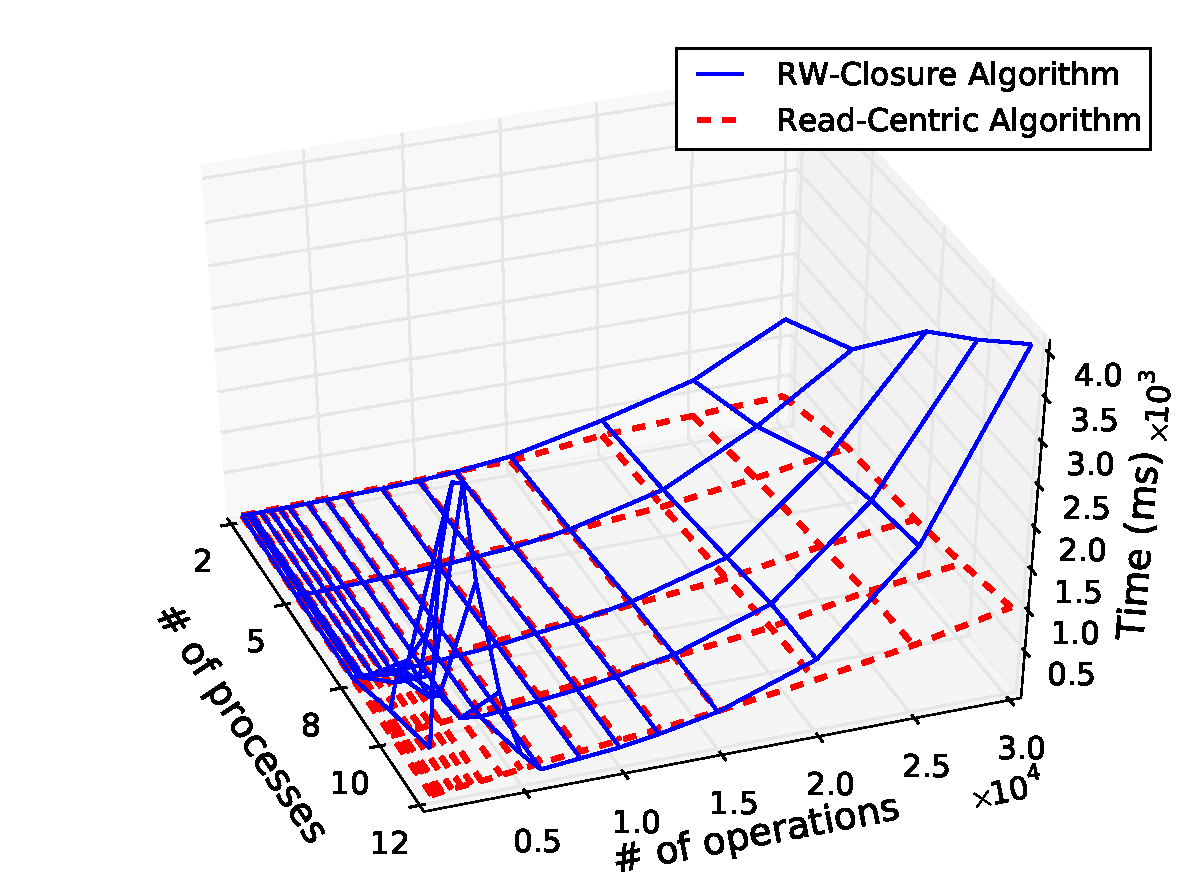
\includegraphics[width = 0.80\textwidth]{figures/vpc-random-cmp.pdf}
	\end{subfigure}%
	~
	\begin{subfigure}[t]{0.50\textwidth}
	  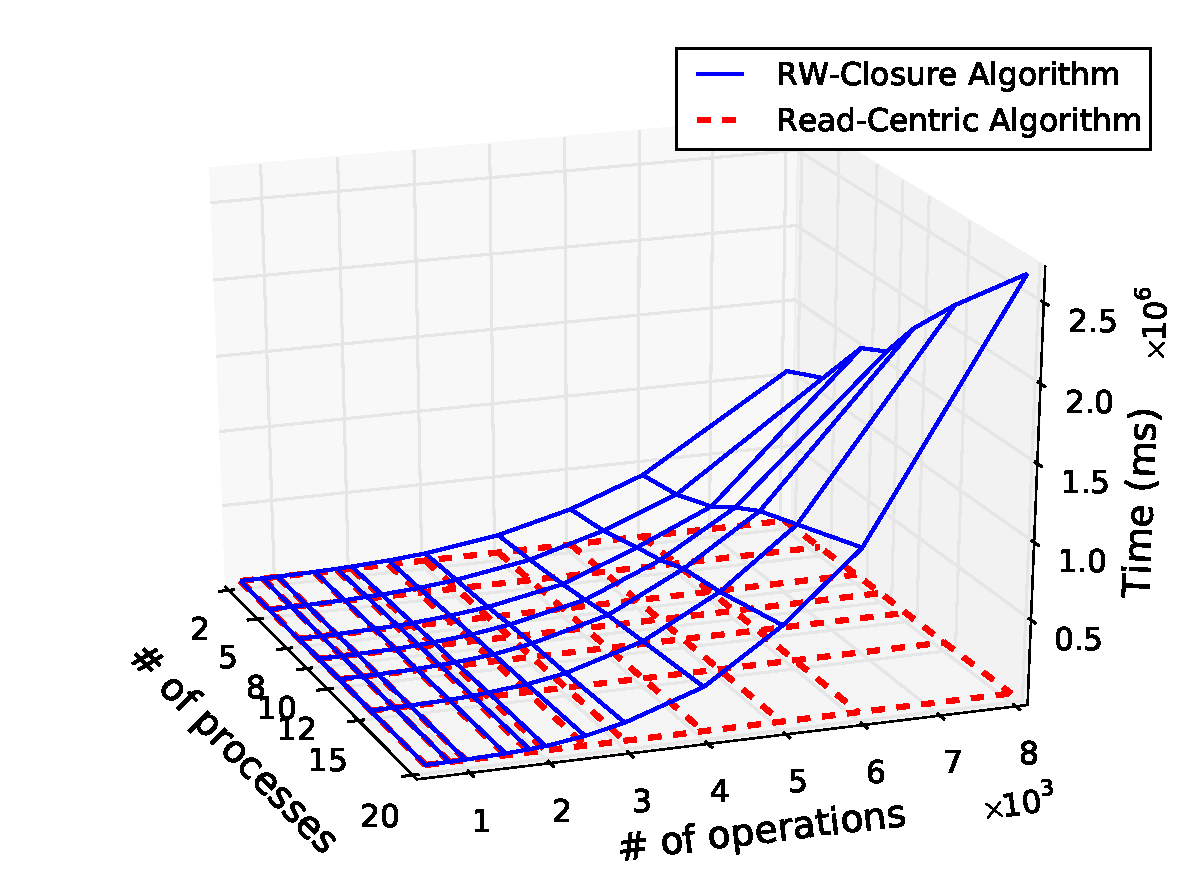
\includegraphics[width = 0.80\textwidth]{figures/vpc-valid-cmp.pdf}
	\end{subfigure}
	\caption{\rwclosure{} 算法与 \readcentric{} 算法在
	\textcolor{blue!80}{ (左) 随机生成}的执行及
	\textcolor{red!80}{ (右) 满足 \PRAM{} 一致性}的执行上的运行时间。}
  \end{figure}

  \pause
  \begin{center}
	\textcolor{red}{(右)} 20个进程、8,000 个操作: 

	\readcentric{} 可获得 694 倍加速.
  \end{center}
\end{frame}
%%%%%%%%%%%%%%%
\begin{frame}{实验评估}
  \fig{width = 0.50\textwidth}{figures/vpc-scalability-more.pdf}
  {\readcentric{} 算法在满足 \PRAM{} 一致性的执行上的运行时间.}

  \begin{description}
	\centering
	\item[\readcentric{}:] 20个进程、60,000个操作 < 600s
	\item[\rwclosure{}:] 20个进程、8,000个操作 > 3,000s
  \end{description}
\end{frame}
%%%%%%%%%%%%%%%
\begin{frame}{VPC 的意义}
  \mdf{red}{blue}{对 VPC 问题的系统研究}{teal}{
	\begin{enumerate}
	  \item \readcentric{} 算法可用于测试系统是否正确实现了 \PRAM{} 一致性模型
	  \item \npcn{} 结果有助于理解弱一致性模型的复杂度
	\end{enumerate}
  }
\end{frame}
%%%%%%%%%%%%%%%

%%%%%%%%%%%%%%%%%%%%%%%%%%%%%%%%%%%%%%%%	
\subsection{PA2AM: (2-)Atomicity 一致性维护与量化}

%%%%%%%%%%%%%%%
\begin{frame}{PA2AM 工作在技术框架中的位置}
  \fig{width = 0.50\textwidth}{figures/3d-framework-pa2am.pdf}{PA2AM --- (2-)Atomicity 一致性维护与量化.}
\end{frame}
%%%%%%%%%%%%%%%
\begin{frame}{研究动机}
  \question{问题: 为什么提出 probabilistically-atomic 2-atomicity {\small (PA2AM)} 一致性?}
  \vspace{0.30cm}

  \pause
  ``数据一致性/访问延迟'' PACELC 权衡 \citeinbeamer{Abadi}{IEEE Computer}{12}:

  \fignocaption{width = 0.35\textwidth}{figures/stronger-consistency-tradeoff.pdf}

  % \begin{quote}
  %   ``As soon as a distributed storage system replicates data, a \textcolor{brown}{tradeoff 
  %   between consistency and latency} arises.''
  % \end{quote}

  \pause

  ``低延迟''至关重要:
  \begin{itemize}
	\item 100ms 额外延迟 $\Rightarrow$ 1\% 销售下滑 \citeinbeamer{Amazon}{Blog}{06}
	\item 100$\sim$400ms 额外延迟 $\Rightarrow$ 0.2\%$\sim$0.6\% 搜索量下降 \citeinbeamer{Google}{Blog}{09}
  \end{itemize}

  % {\small
  % \begin{table}
  %   \begin{tabular}{c|c}
  %     \textcolor{blue}{\bf 系统} & \textcolor{blue}{\bf 一致性}		\\ \hline
  %     Dynamo@Amazon \citeinbeamer{Amazon}{SOSP}{07} & eventual consistency \\ \hline
  %     PNUTS@Yahoo! \citeinbeamer{Yahoo!}{PVLDB}{08} & cache consistency \\ \hline
  %     Tao@Facebook \citeinbeamer{Facebook}{ATC}{13} & $\le$ read-after-write \\ \hline
  %   \end{tabular}
  % \end{table}
  % }
\end{frame}
%%%%%%%%%%%%%%%
\begin{frame}{PA2AM 一致性}
  % \begin{cdef}[``近乎强''一致性]
  %   对某特定强一致性的弱化: \begin{itemize}
  %     \item (版本) 允许读陈旧值,但陈旧度有限
  %     \item (概率) 读到陈旧值的概率很小
  %   \end{itemize}
  % \end{cdef}

  \begin{center}
	\only<2->{\textcolor{blue}{``近乎强''一致性: }}{在保证\textcolor{red}{低延迟}的情况下获得\textcolor{red}{尽可能强}的数据一致性.}
  \end{center}

  \uncover<3->{
  \begin{cdef}[PA2AM 一致性]
	\begin{description}
	  \setlength{\itemsep}{5pt}
	  \item[低延迟:] \uncover<4->{读操作只需一轮网络通信} 
	  \item[尽可能强:] \uncover<6->{对 atomicity {\small (strongest)} 的弱化}
    \begin{itemize}
	  \item<6-> \textcolor{brown}{\it (版本)} 2-atomicity: 允许读陈旧值, 但\textcolor{red}{陈旧度 $k \le 2$}
	  \item<6-> \textcolor{brown}{\it (概率)} \textcolor{red}{$\mathbb{P}(k = 2)$ 很小}
    \end{itemize}
    \end{description}
  \end{cdef}
  }

  \vspace{0.20cm}
  \uncover<5->{
  \begin{ctheorem}[不可能性结果]
    (单写模型下) 不存在低延迟的 atomicity 维护算法 \citeinbeamer{Dutta}{PODC}{04}.
  \end{ctheorem}
  }
\end{frame}
%%%%%%%%%%%%%%%
\begin{frame}{PA2AM 维护算法}
  \fig{width = 0.80\textwidth}{figures/atomicity-2am-read-compare.pdf}
  {经典 atomicity 算法中, 读操作需两轮网络通信 \citeinbeamer{Attiya}{JACM}{95} 
  \citeinbeamer{Dutta}{PODC}{04}. 
  PA2AM 算法实现 2-atomicity {\scriptsize (单写模型下)}, 读操作只需一轮网络通信.}
\end{frame}
%%%%%%%%%%%%%%%
\begin{frame}{PA2AM 量化分析}
  \question{问题: PA2AM 算法在多大程度上违反了 atomicity?}
  \vspace{0.10cm}

  \begin{itemize}
    \setlength{\itemsep}{10pt}
	\item 充要条件: ONI (old-new inversion) \citeinbeamer{Attiya}{JACM}{95}
      \fignocaption{width = 0.45\textwidth}{figures/2atomicity-case.pdf}
    \item PA2AM 量化分析: 计算 $\mathbb{P}(\textrm{ONI})$, 其值越小越好
      \begin{enumerate}
        \setlength{\itemsep}{3pt}
        \item $\textrm{ONI} \triangleq \textrm{CP} \cap \textrm{RWP}$
        \item 排队论建模, 计算 $\mathbb{P}(\textrm{CP})$ \item 带时间的球盒模型, 计算 
          $\mathbb{P}(\textrm{RWP|CP})$
        % \item 实验统计 $\mathbb{P}(\textrm{CP})$, $\mathbb{P}(\textrm{RWP|CP})$ 与 
        % $\mathbb{P}(\textrm{ONI})$, 以作对照
      \end{enumerate}
  \end{itemize}
\end{frame}
%%%%%%%%%%%%%%%
\begin{frame}{PA2AM 量化分析}
  公式推导:
  \begin{figure}
	\begin{subfigure}{0.50\textwidth}
	  \centering
	  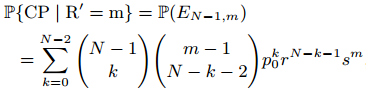
\includegraphics[width = 0.70\textwidth]{figures/cp.png}
	\end{subfigure}%
	\begin{subfigure}{0.50\textwidth}
	  \centering
	  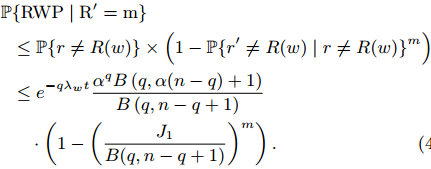
\includegraphics[width = 0.70\textwidth]{figures/rwp.png}
	\end{subfigure}
  \end{figure}

  \vspace{0.10cm}

  数值结果 (左一) 与实验结果 (右二): 
  \begin{figure}
	\begin{subfigure}{0.45\textwidth}
	  \centering
	  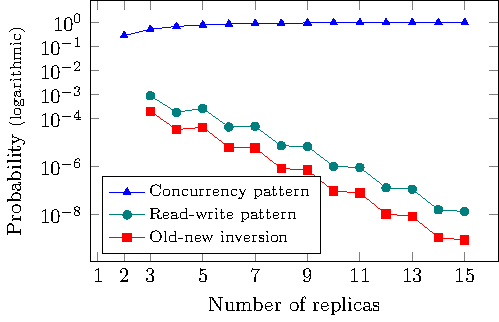
\includegraphics[width = 0.60\textwidth]{figures/oni-pgfplot.pdf}
	\end{subfigure}%
	\begin{subfigure}{0.55\textwidth}
	  \centering
	  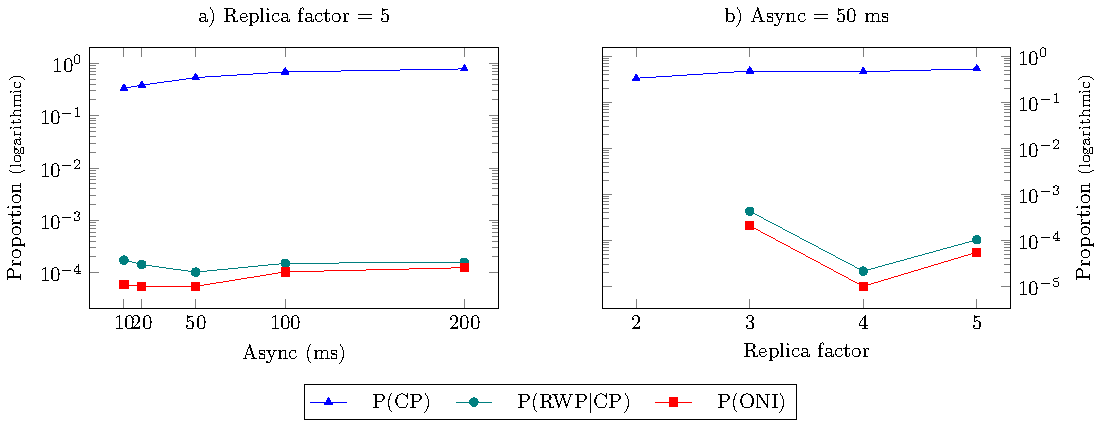
\includegraphics[width = 0.90\textwidth]{figures/experiment-oni-pgfplot.pdf}
	\end{subfigure}
  \end{figure}
\end{frame}
%%%%%%%%%%%%%%%
\begin{frame}{PA2AM vs. 弱一致性模型}
  \begin{figure}
	\begin{subfigure}{0.50\textwidth}
	  \centering
	  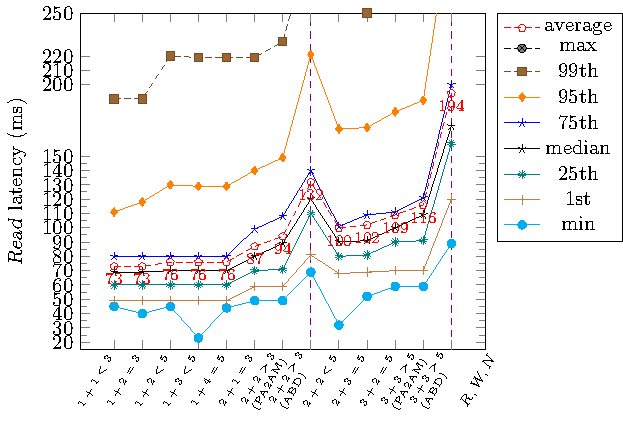
\includegraphics[width = 0.85\textwidth]{figures/rwn-2am-read-latency-quantiles.pdf}
	  \caption{读操作延迟对比.}
	\end{subfigure}%
	\begin{subfigure}{0.50\textwidth}
	  \centering
	  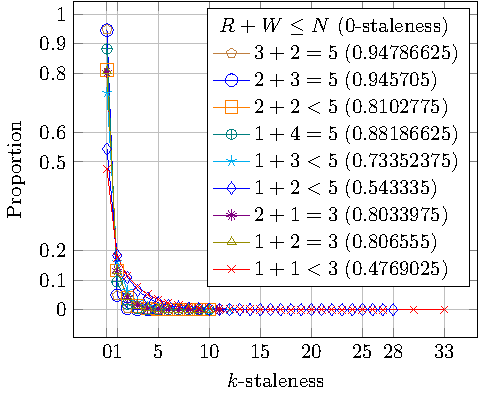
\includegraphics[width = 0.70\textwidth]{figures/rwn-maj.pdf}
	  \caption{$k$-陈旧度对比.}
	\end{subfigure}
	\caption{PA2AM 与 eventual consistency (RWN-Maj 协议) 对比结果.}
  \end{figure}

  \vspace{-0.50cm}
  \begin{table}[]
  \renewcommand{\arraystretch}{1.3}
  \centering
  \caption{不同 $R,W,N$ 配置下, RWN-All 执行中具有不同陈旧度的读操作的比率.}
  \label{tbl:rwn-all-staleness}
  \resizebox{\textwidth}{!}{%
  \begin{tabular}{|c||c|c|c|c||c|c|c|c|c|c|c|}
  \hline
  {\bfseries \# replicas} & \multicolumn{4}{c||}{\bfseries replica factor = 3 ($400,000$
    \textsl{read} operations)} & \multicolumn{7}{c|}{\bfseries replica factor = 5 ($800,000$
    \textsl{read} operations)} 
  \\ \hline
  {\bfseries $R,W,N$} % \textrm{R}+\textrm{W} $\boldsymbol{\le}$ \textrm{N}}  
  & $1+1<3$	& $1+2=3$	& $2+1=3$	& $2+2>3 \;(\text{PA2AM})$ 
  & $1+2<5$ 	& $1+3<5$ 	& $1+4=5$	& $2+2<5$ 	& $2+3=5$    & $3+2=5$     & $3+3>5 \;(\text{PA2AM})$     
  \\ \hline \hline
  {\boldmath $\max k$}          & $6$      & $4$ 	& $2$    &  {\boldmath $1$}
  & $2$	& $2$      	& $2$	   & $2$	& $2$	 &  $2$     & {\boldmath $1$}
  \\ \hline
  {\bfseries $\sum_{k \ge 1}$-staleness}       & $0.0084125$      & $0.000315$ 	&  $0.0004675$	&
  {\boldmath $0.000085$}
  	&  $0.00377875$	&  $0.002755$	&  $0.00406$     & $0.0027225$      & $0.0020275$     & $0.002255$      
	&  {\boldmath $0.0003525$}
  \\ \hline
  \end{tabular}%
}
\end{table}

\end{frame}
%%%%%%%%%%%%%%%
\begin{frame}{PA2AM 的意义}
  \mdf{red}{blue}{PA2AM 可作为一致性/延迟权衡的一种有价值的选项}{teal}{
	\begin{itemize}
	  \item 既 {\small (在统计意义上)} 满足强一致性模型对数据一致性的高标准
	  \item 又具有弱一致性模型的性能优势
    \end{itemize}
  }
\end{frame}
%%%%%%%%%%%%%%%

%%%%%%%%%%%%%%%%%%%%%%%%%%%%%%%%%%%%%%%%	
\subsection{RVSI: Snapshot Isolation 一致性弱化与维护}

\newcommand{\chameleon}{\textsc{Chameleon}}
\newcommand{\konebv}{$k_1$-BV}
\newcommand{\ktwofv}{$k_2$-FV}
\newcommand{\kthreesv}{$k_3$-SV}
%%%%%%%%%%%%%%%
\begin{frame}{RVSI 工作在技术框架中的位置}
  \fig{width = 0.50\textwidth}{figures/3d-framework-rvsi.pdf}
	{RVSI --- Snapshot Isolation 一致性弱化与维护.}
\end{frame}
%%%%%%%%%%%%%%%
\begin{frame}{研究动机}
  \question{问题: 为什么要提出 Relaxed Version Snapshot Isolation {\small (RVSI)} 一致性?}
  \vspace{0.20cm}

  \begin{description}
    \setlength{\itemsep}{5pt}
    \item[分布式事务:]
      \begin{itemize}
        \item ``all-or-none'' 语义
        \item 受到分布式存储系统的关注 \citeinbeamer{Cassandra}{CASSANDRA-ISSUE-7056}{14}
      \end{itemize}
    \item[弱一致性:] 
        PCSI \citeinbeamer{Elnikety}{SRDS}{05} 
		  \textcolor{red}{SI} \citeinbeamer{Lin}{TODS}{09} \\
          PSI \citeinbeamer{Sovran}{SOSP}{11} NMSI \citeinbeamer{Ardekani}{SRDS}{13} 
    \pause
	\item[\textcolor{red}{异常控制:}] 容忍``有限度的''异常 \citeinbeamer{Yu}{TOCS}{02}
	\item[\textcolor{red}{可调节:}] 
      \begin{itemize}
        \item 不同应用对一致性需求不同 \citeinbeamer{Terry}{CACM}{13}
        \item 运行时决定 \citeinbeamer{Terry}{SOSP\&TR}{13}
      \end{itemize}
  \end{description}
\end{frame}
%%%%%%%%%%%%%%%
\begin{frame}{RVSI 定义}
  RVSI 定义原则:
  \begin{itemize}
    \item 参数 $k_1, k_2, k_3$ 控制``异常''程度
    \item $\text{RC} \supset \text{RVSI}(k_1, k_2, k_3) \supset \text{SI}$
    \item $\text{RVSI}(\infty,\infty,\infty) = \text{RC}; \qquad \text{RVSI}(1,0,\ast) = \text{SI}$
  \end{itemize}

  \vspace{0.20cm}

  \begin{cdef}[RVSI: Relaxed Version Snapshot Isolation]
    \begin{description}
      \item[单变量读 $\texttt{read}(x)$:] \hfill 
        \begin{enumerate}
		  \item 允许读 $\le k_1$ 陈旧值 (\konebv{})
		  \item 允许读 $\le k_2$ 并发更新 (\ktwofv{})
        \end{enumerate}
      \item[多变量读 $\texttt{read}(x), \texttt{read}{(y)}$:] \hfill
        \begin{enumerate}
          \setcounter{enumi}{2}
		\item $\text{distance}(\textsl{snap}{(x)},\textsl{snap}{(y)}) \le k_3$
        \end{enumerate}
    \end{description}
  \end{cdef}
\end{frame}
%%%%%%%%%%%%%%%
\begin{frame}{\chameleon{} 分布式事务键值存储原型系统设计}
  \begin{description}
	\item[系统架构:] 阿里云\footnote{阿里云: \url{https://www.aliyun.com/}.} 
	  多数据中心 {\small ($9 = 3 \times 3$)}
	\item<2->[数据分区:] 同一数据中心
	\item<2->[数据副本:] 跨数据中心; 主从结构
  \end{description}

  \fignocaption{width = 0.55\textwidth}{figures/chameleon-arch.pdf}
\end{frame}
%%%%%%%%%%%%%%%
\begin{frame}{\chameleon{} 分布式事务键值存储原型系统设计}
  \begin{description}
	\item[系统组件:] 客户端库 + 数据中心
	\item<2->[数据分区:] 分布式事务原子提交协议 {\small (2PC)}
	\item<2->[数据副本:] 懒惰复制 {\small (lazy replication)} 协议
  \end{description}

  \fignocaption{width = 0.42\textwidth}{figures/chameleon-framework.pdf}
\end{frame}
%%%%%%%%%%%%%%%
\begin{frame}{RVSI 维护算法}
  \[
    \textcolor{blue}{\text{RC} \supset \text{RVSI}(k_1, k_2, k_3) \supset \text{SI}}
  \]

  \vspace{0.10cm}

  RVSI 维护算法:
  \begin{itemize}
    \item 以分布式 RC 和 SI 协议 为基础
    \item 事务执行时, 添加 RVSI ``版本约束'' ($k_1, k_2, k_3$ 相关不等式)
    \item 事务提交时, 检查 RVSI ``版本约束''
  \end{itemize}

  % \fignocaption{width = 0.50\textwidth}{figures/chameleon-build-passing.png}
  \textcolor{red}{\small \url{https://github.com/hengxin/chameleon-transactional-kvstore}}
\end{frame}
%%%%%%%%%%%%%%%
\begin{frame}{RVSI 实验评估}
  \begin{table}[]
  \renewcommand{\arraystretch}{1.1}
  \centering
  \caption{事务负载参数表.\protected\\(\textcolor{blue}
	{评估目标: RVSI 对事务中止率的影响})}
  \resizebox{\textwidth}{!}{%
  \begin{tabular}{|c||c|c|c|}
	\hline
	{\bfseries Parameter}   & {\bfseries F(ixed)/V(ariable)/R(andom)}	
	& {\bfseries Value}		& {\bfseries Explanation}
	\\ \hline  \hline
	\#keys  				& F		& 5  				&  	size of keyspace
	\\ \hline
	\cellcolor{brown}mpl	& \textcolor{red}{\bf V}		& 5, 10, 15, 20, 25, 30
	& \innercell{c}{multiprogramming level: \\ number of concurrent clients} \\ \hline
	\#txs/client					& F		& 1000 						
	& \innercell{c}{number of txs per client}
	\\ \hline
	\#ops/tx					& R		& $\sim$ Binomial(20, 0.5)	
	&  \innercell{c}{number of operations per tx}
	\\ \hline
	\cellcolor{brown}rwRatio & \textcolor{red}{\bf V} 
	  & 1:2, 1:1, 4:1 & {\#reads}/{\#writes}
	\\ \hline
	zipfExponent			& F		& 1		& parameter for Zipfian distribution
	\\ \hline  \hline
	\cellcolor{brown}$(k_1, k_2, k_3)$		& \textcolor{red}{\bf V}
		&  \innercell{c}{(1,0,0) \\ (1,0,2) (1,1,0) \\ (2,0,0) (2,1,2) (2,2,1)}	
		&  for \konebv{}, \ktwofv{}, and \kthreesv{}
	\\ \hline  \hline
	minInterval				& F		& 0ms		& minimum inter-transactions time
	\\ \hline
	maxInterval				& F		& 10ms		& maximum inter-transactions time
	\\ \hline
	meanInterval			& R		& 5ms		
	& \innercell{c}{mean inter-transactions time \\ for exponential distribution}
	\\ \hline
  \end{tabular}
  }
\end{table}

\end{frame}
%%%%%%%%%%%%%%%
\begin{frame}{RVSI 实验评估}
  \fig{width = 0.70\textwidth}{figures/rvsi-rw4-abort-rates.pdf}
	{读频繁 (rwRatio = 4:1) 负载下 RVSI 对事务中止率的影响.}

  \begin{description}
	\item[\textcolor{blue}{wcf-aborted:}] 
	  无显著变化 {\small ($\text{wcf}(1,0,0) = 0.184733$)}
	\item[\textcolor{red}{vc-aborted:}] 显著减少 
	  {\small ($\text{vc}(1,0,0) = 0.204733;
	  \text{vc}(1,1,0) = 0.066433;
	  \text{vc}(2,2,1) = 0.002033$)}
  \end{description}
\end{frame}
%%%%%%%%%%%%%%%
\begin{frame}{RVSI 实验评估}
  \begin{columns}
	\column{0.48\textwidth}
	  \fig{width = 1.00\textwidth}{figures/rvsi-rw05-abort-rates.pdf}
		{写频繁 (rwRatio = 1:2) 负载下 RVSI 对事务中止率的影响.}
	\column{0.48\textwidth}
	  \fig{width = 1.00\textwidth}{figures/rvsi-rw1-abort-rates.pdf}
		{读写相当 (rwRatio = 1:1) 负载下 RVSI 对事务中止率的影响.}
  \end{columns}
\end{frame}
%%%%%%%%%%%%%%%
\begin{frame}{RVSI 的意义}
  \mdf{red}{blue}{RVSI 对事务中止率的影响}{teal}{
	\begin{enumerate}
	  \item 适当放松事务对 RVSI 版本规约的要求可降低事务中止率
	  \item RVSI 能否``显著''降低事务中止率与负载类型相关
    \end{enumerate}
  }
\end{frame}
%%%%%%%%%%%%%%%

%%%%%%%%%%%%%%%
\begin{frame}{工作总结}
\end{frame}
%%%%%%%%%%%%%%%

% \section{未来工作}

%%%%%%%%%%%%%%%%%%%%%%%%%%%%%%

%%%%%%%%%%%%%%%
\begin{frame}{分布数据一致性问题研究的发展趋势 (I)}
  
\end{frame}
%%%%%%%%%%%%%%%
\begin{frame}{分布数据一致性问题研究的发展趋势 (II)}
  
\end{frame}
%%%%%%%%%%%%%%%
%%%%%%%%%%%%%%%
%%%%%%%%%%%%%%%
%%%%%%%%%%%%%%%
%%%%%%%%%%%%%%%
%%%%%%%%%%%%%%%
%%%%%%%%%%%%%%%


\end{document}